\chapter{Measurement Results}\label{cha:results}
\noindent
\section{Noise Measurements}
For the noise measurement, the threshold was scanned in steps of 1 for a range of high gains,
starting with a gain of 58 and ending with a maximal gain of 62.
\newline
The number of hits was measured for each of the 32 channels of the ASICs within a time interval of \SI{400}{\milli\second}.
The threshold scan was performed for both the ASICs of FPGA 1 and 2.
\newline
The results of the threshold scan are shown for both ASICs of FPGA 1 and 2 for gains 58 to 62 in Figs.~\ref{fig:threshold_scan_58},~\ref{fig:threshold_scan_59},~\ref{fig:threshold_scan_60},~\ref{fig:threshold_scan_61} and~\ref{fig:threshold_scan_62} respectively.

    \begin{figure}[H]
        \centering
        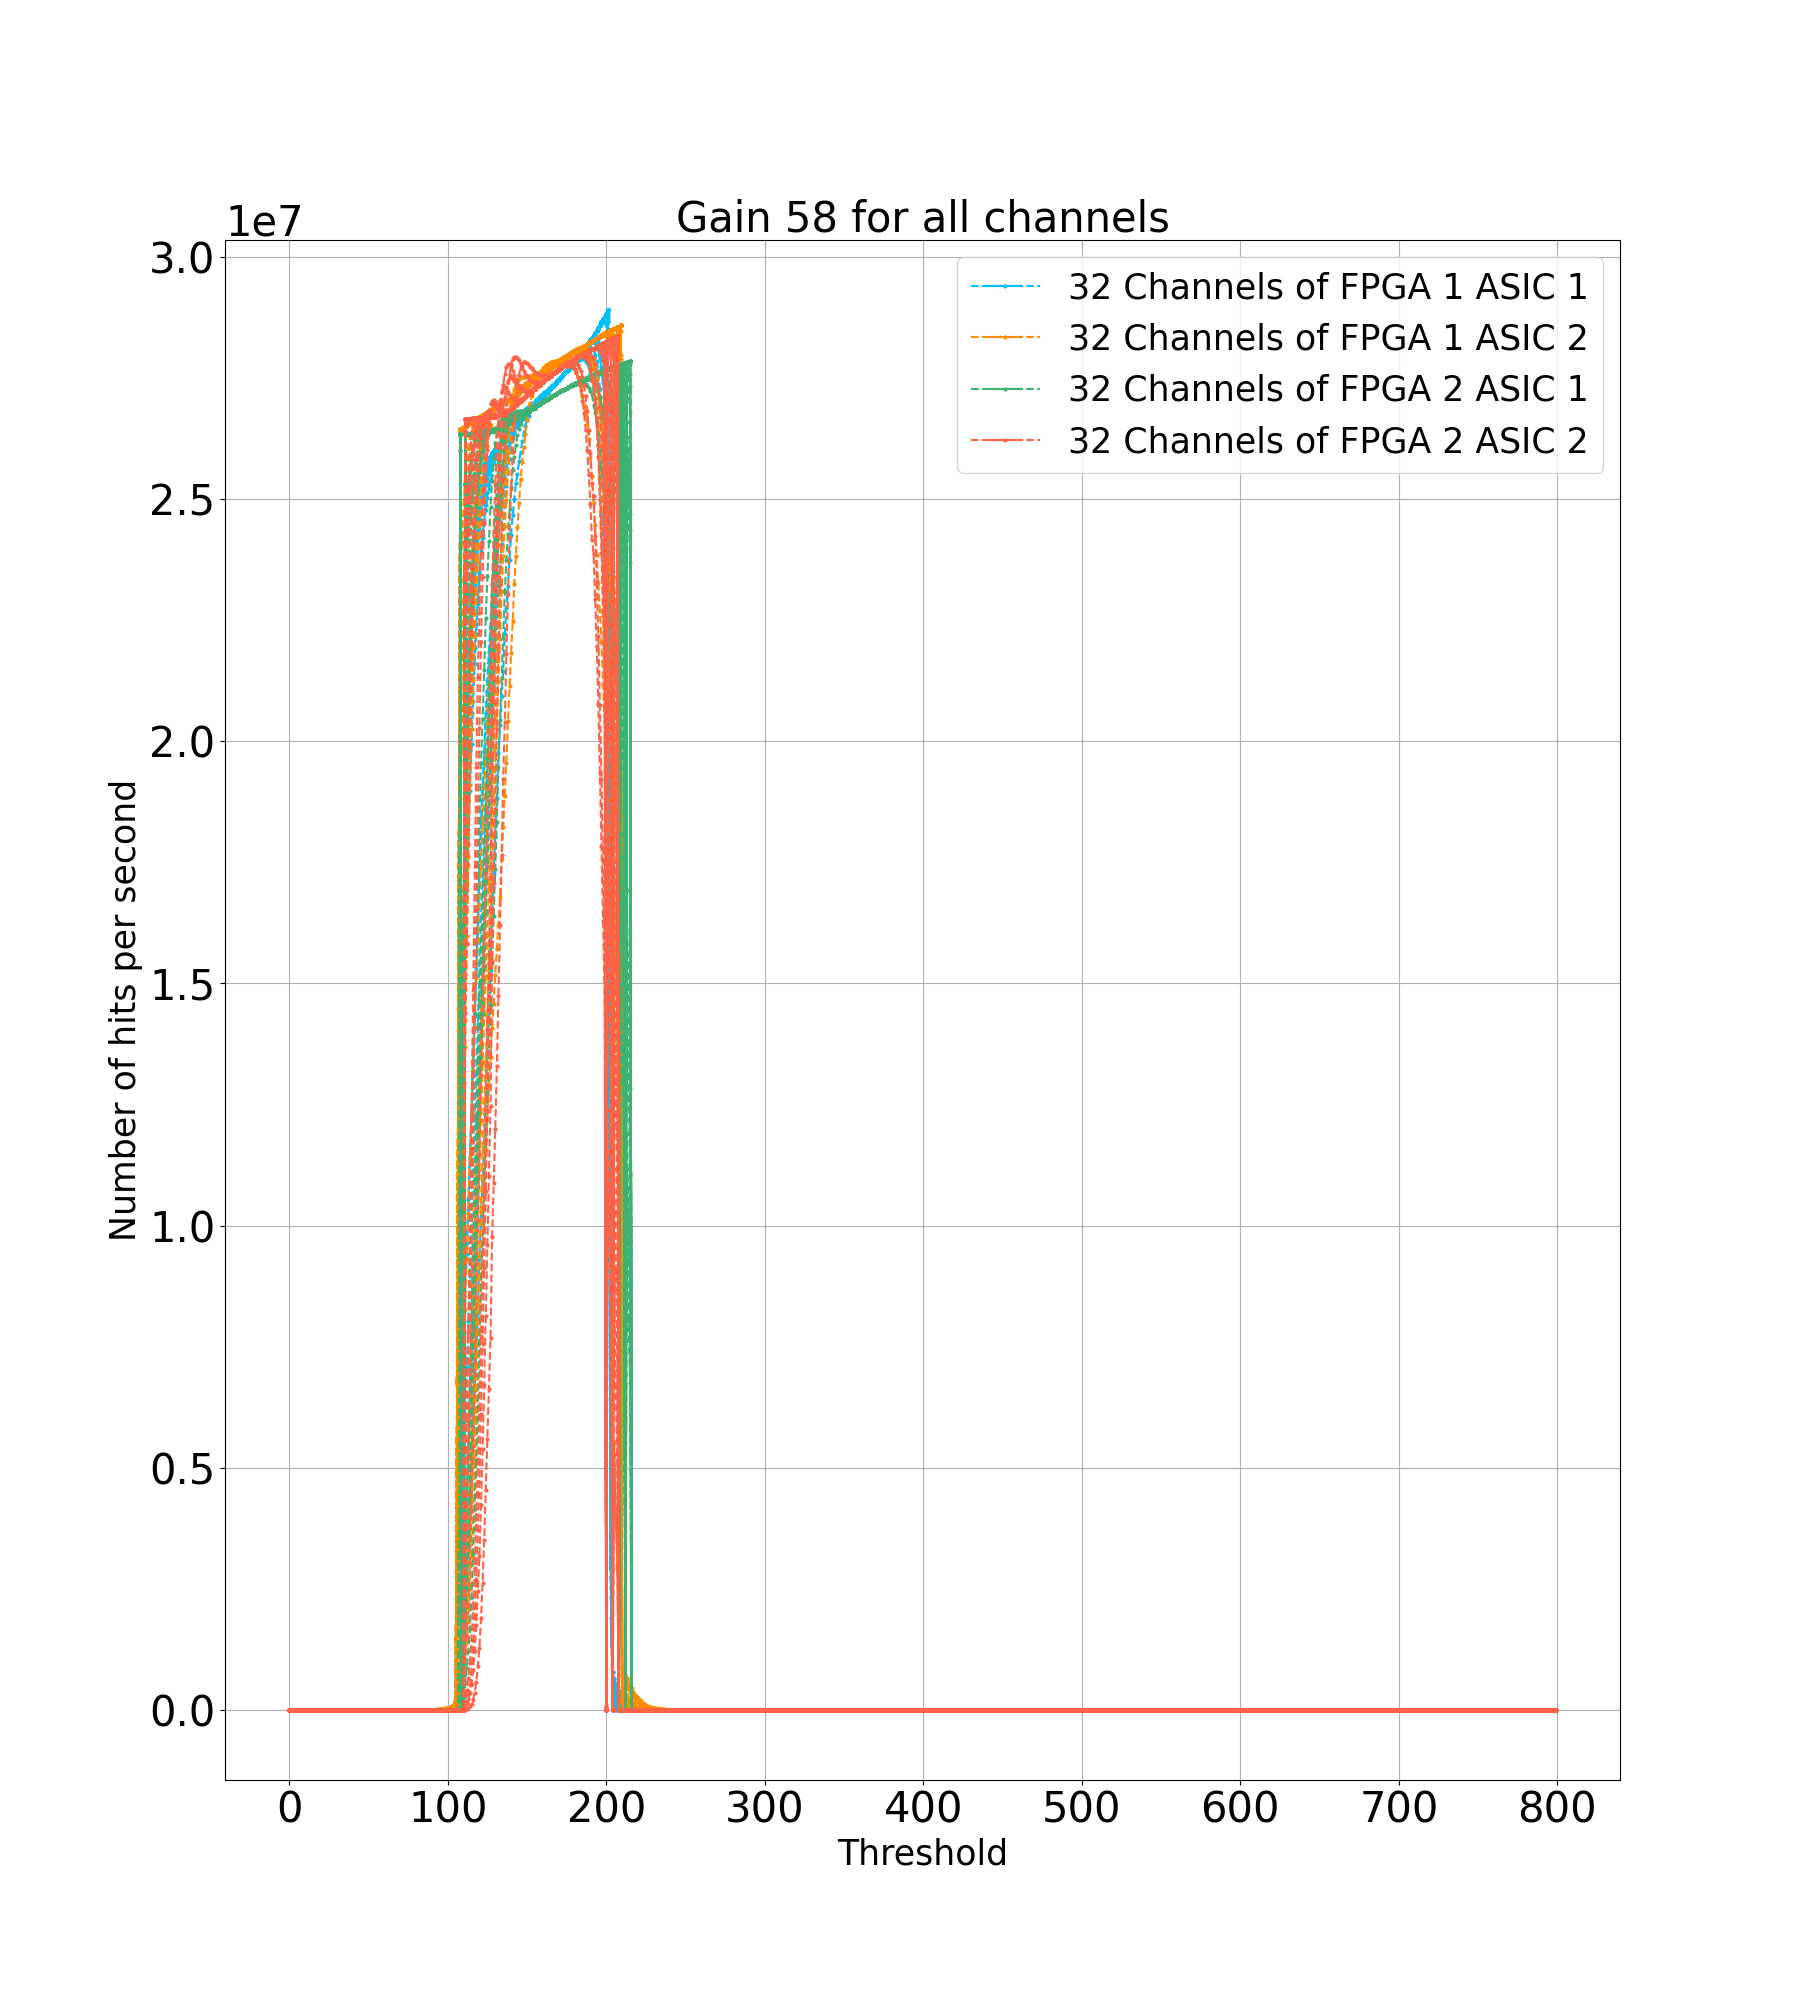
\includegraphics[width=1.0\textwidth]{Gain_58.0_ALLCHANNELS copy 2.png}
        \caption{Threshold scan of the Citiroc1A ASICs of FPGA 1 and 2 for gain 58 from threshold 0 to 800.}
        \label{fig:threshold_scan_58}
    \end{figure}
    
    \begin{figure}[H]
        \centering
        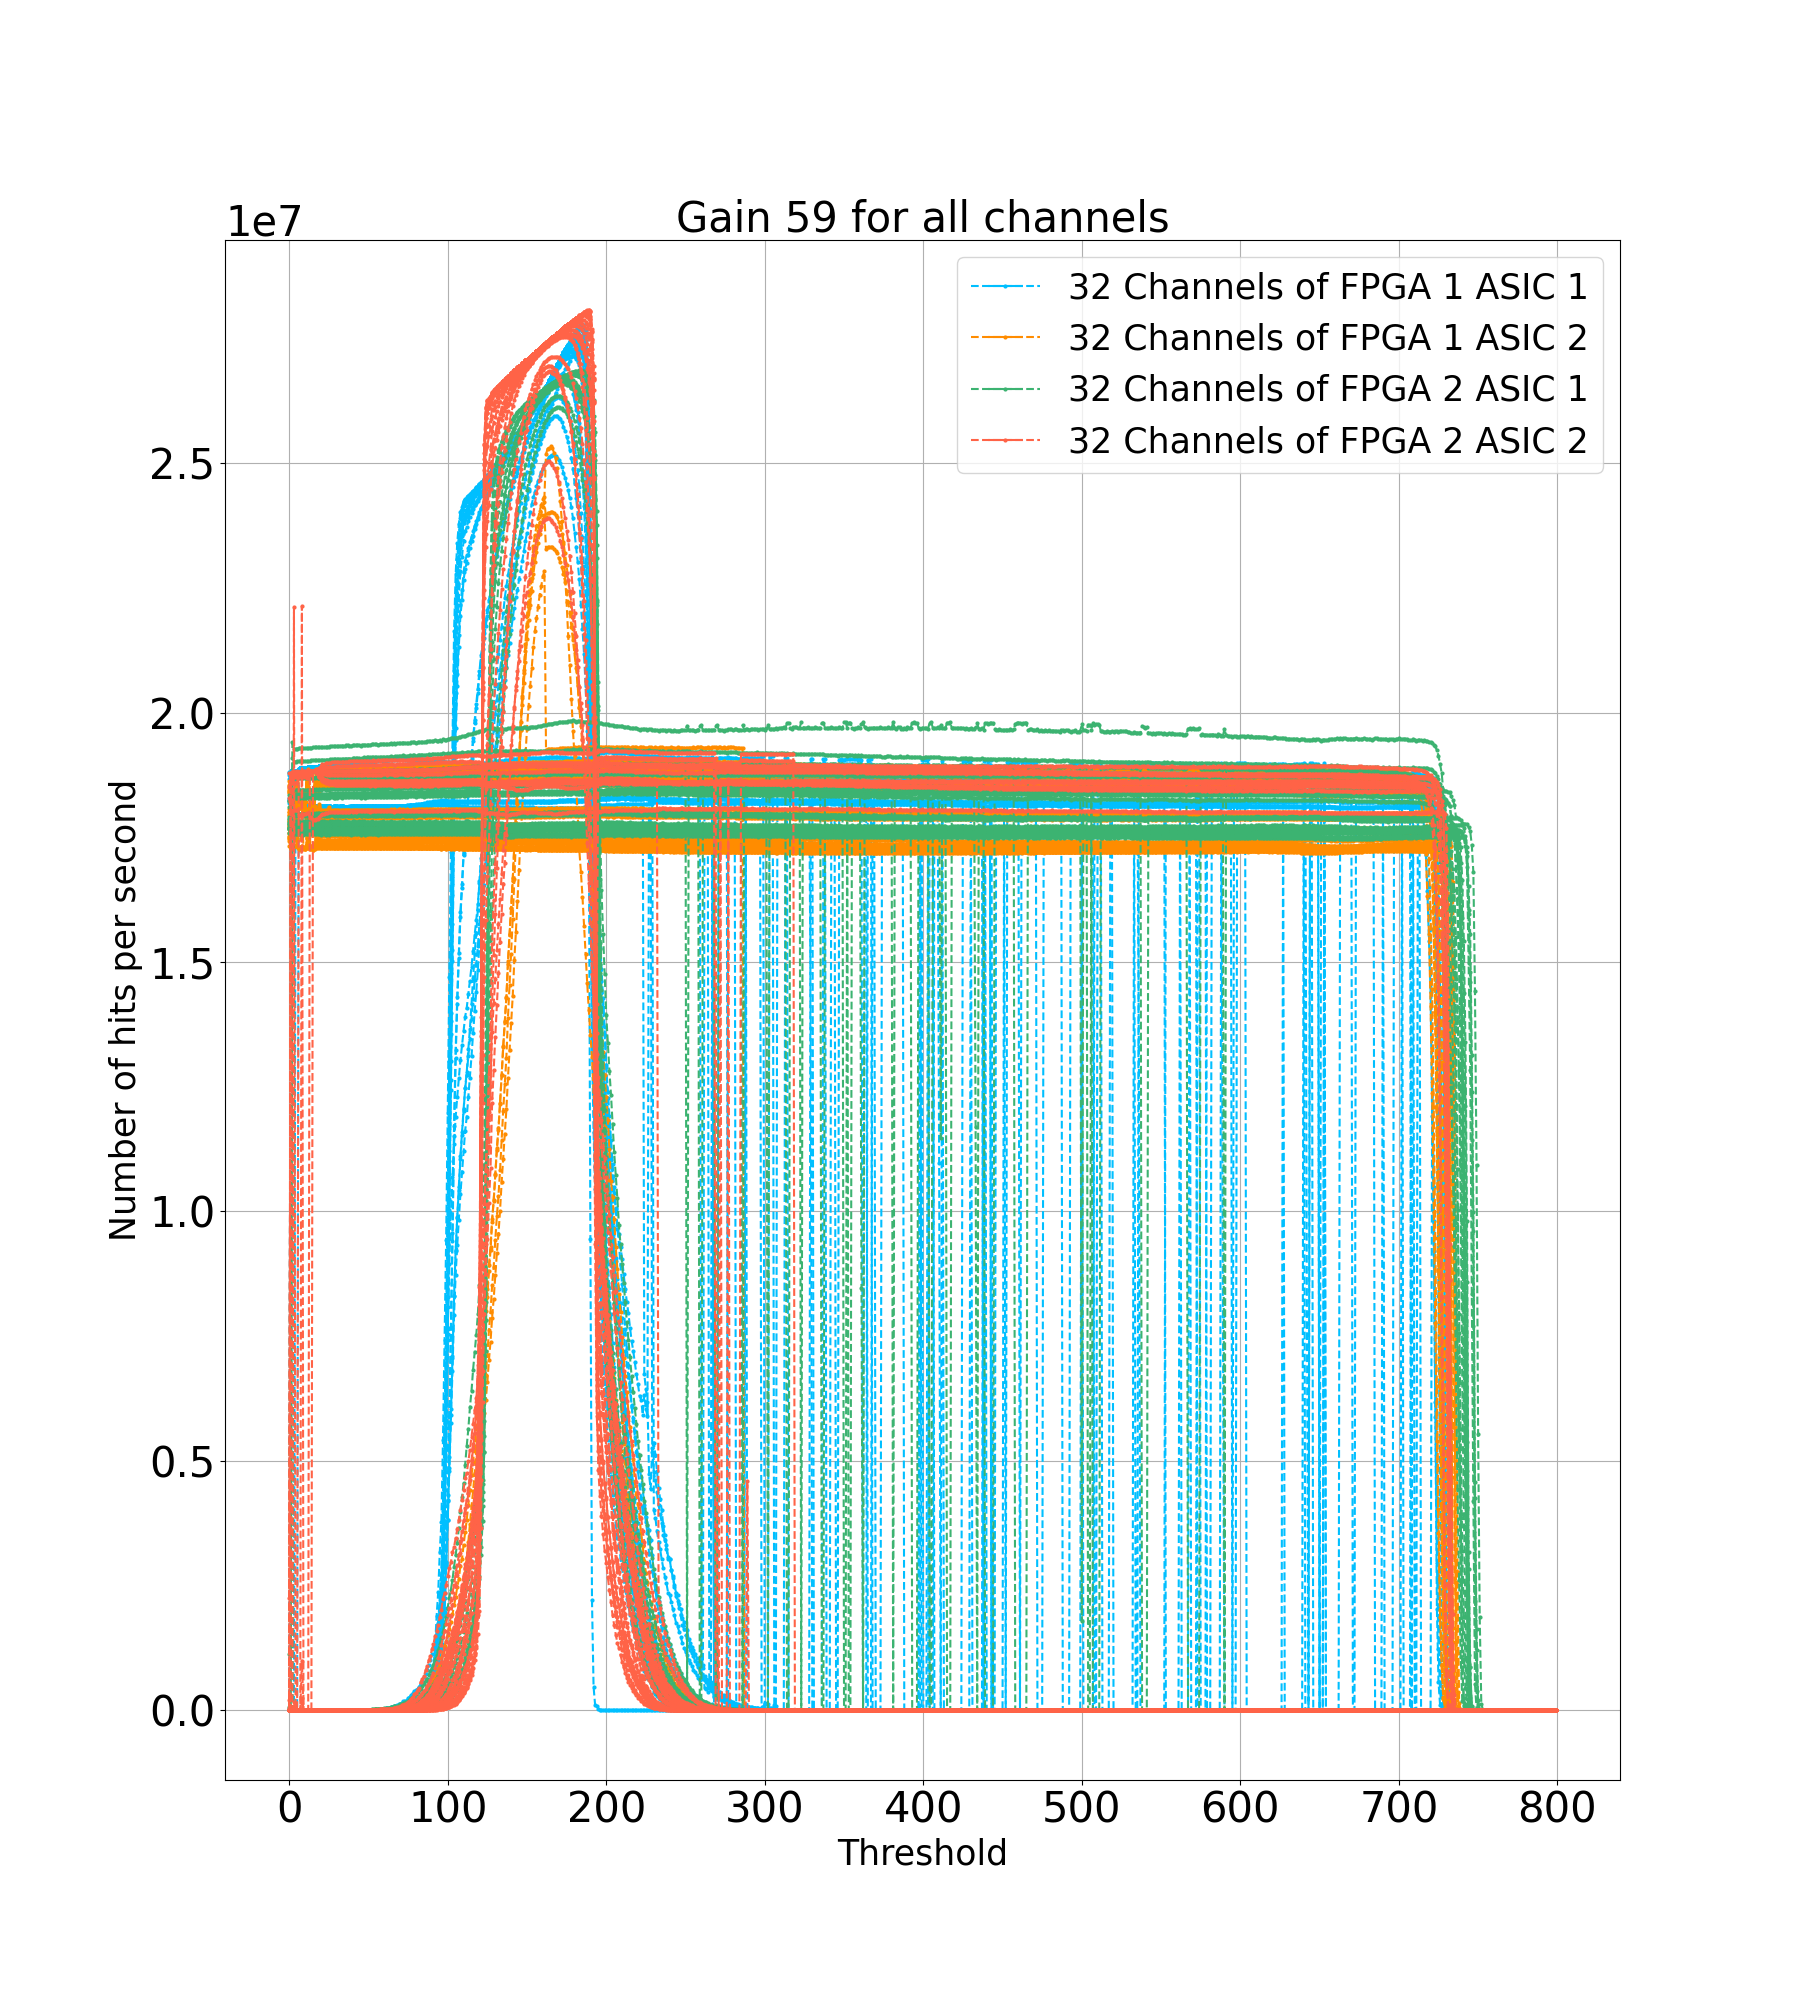
\includegraphics[width=1.0\textwidth]{Gain_59.0_ALLCHANNELS copy 2.png} 
        \caption{Threshold scan of the Citiroc1A ASICs of FPGA 1 and 2 for gain 59 from threshold 0 to 800.}
        \label{fig:threshold_scan_59}
    \end{figure}
    
    \begin{figure}[H]
        \centering
        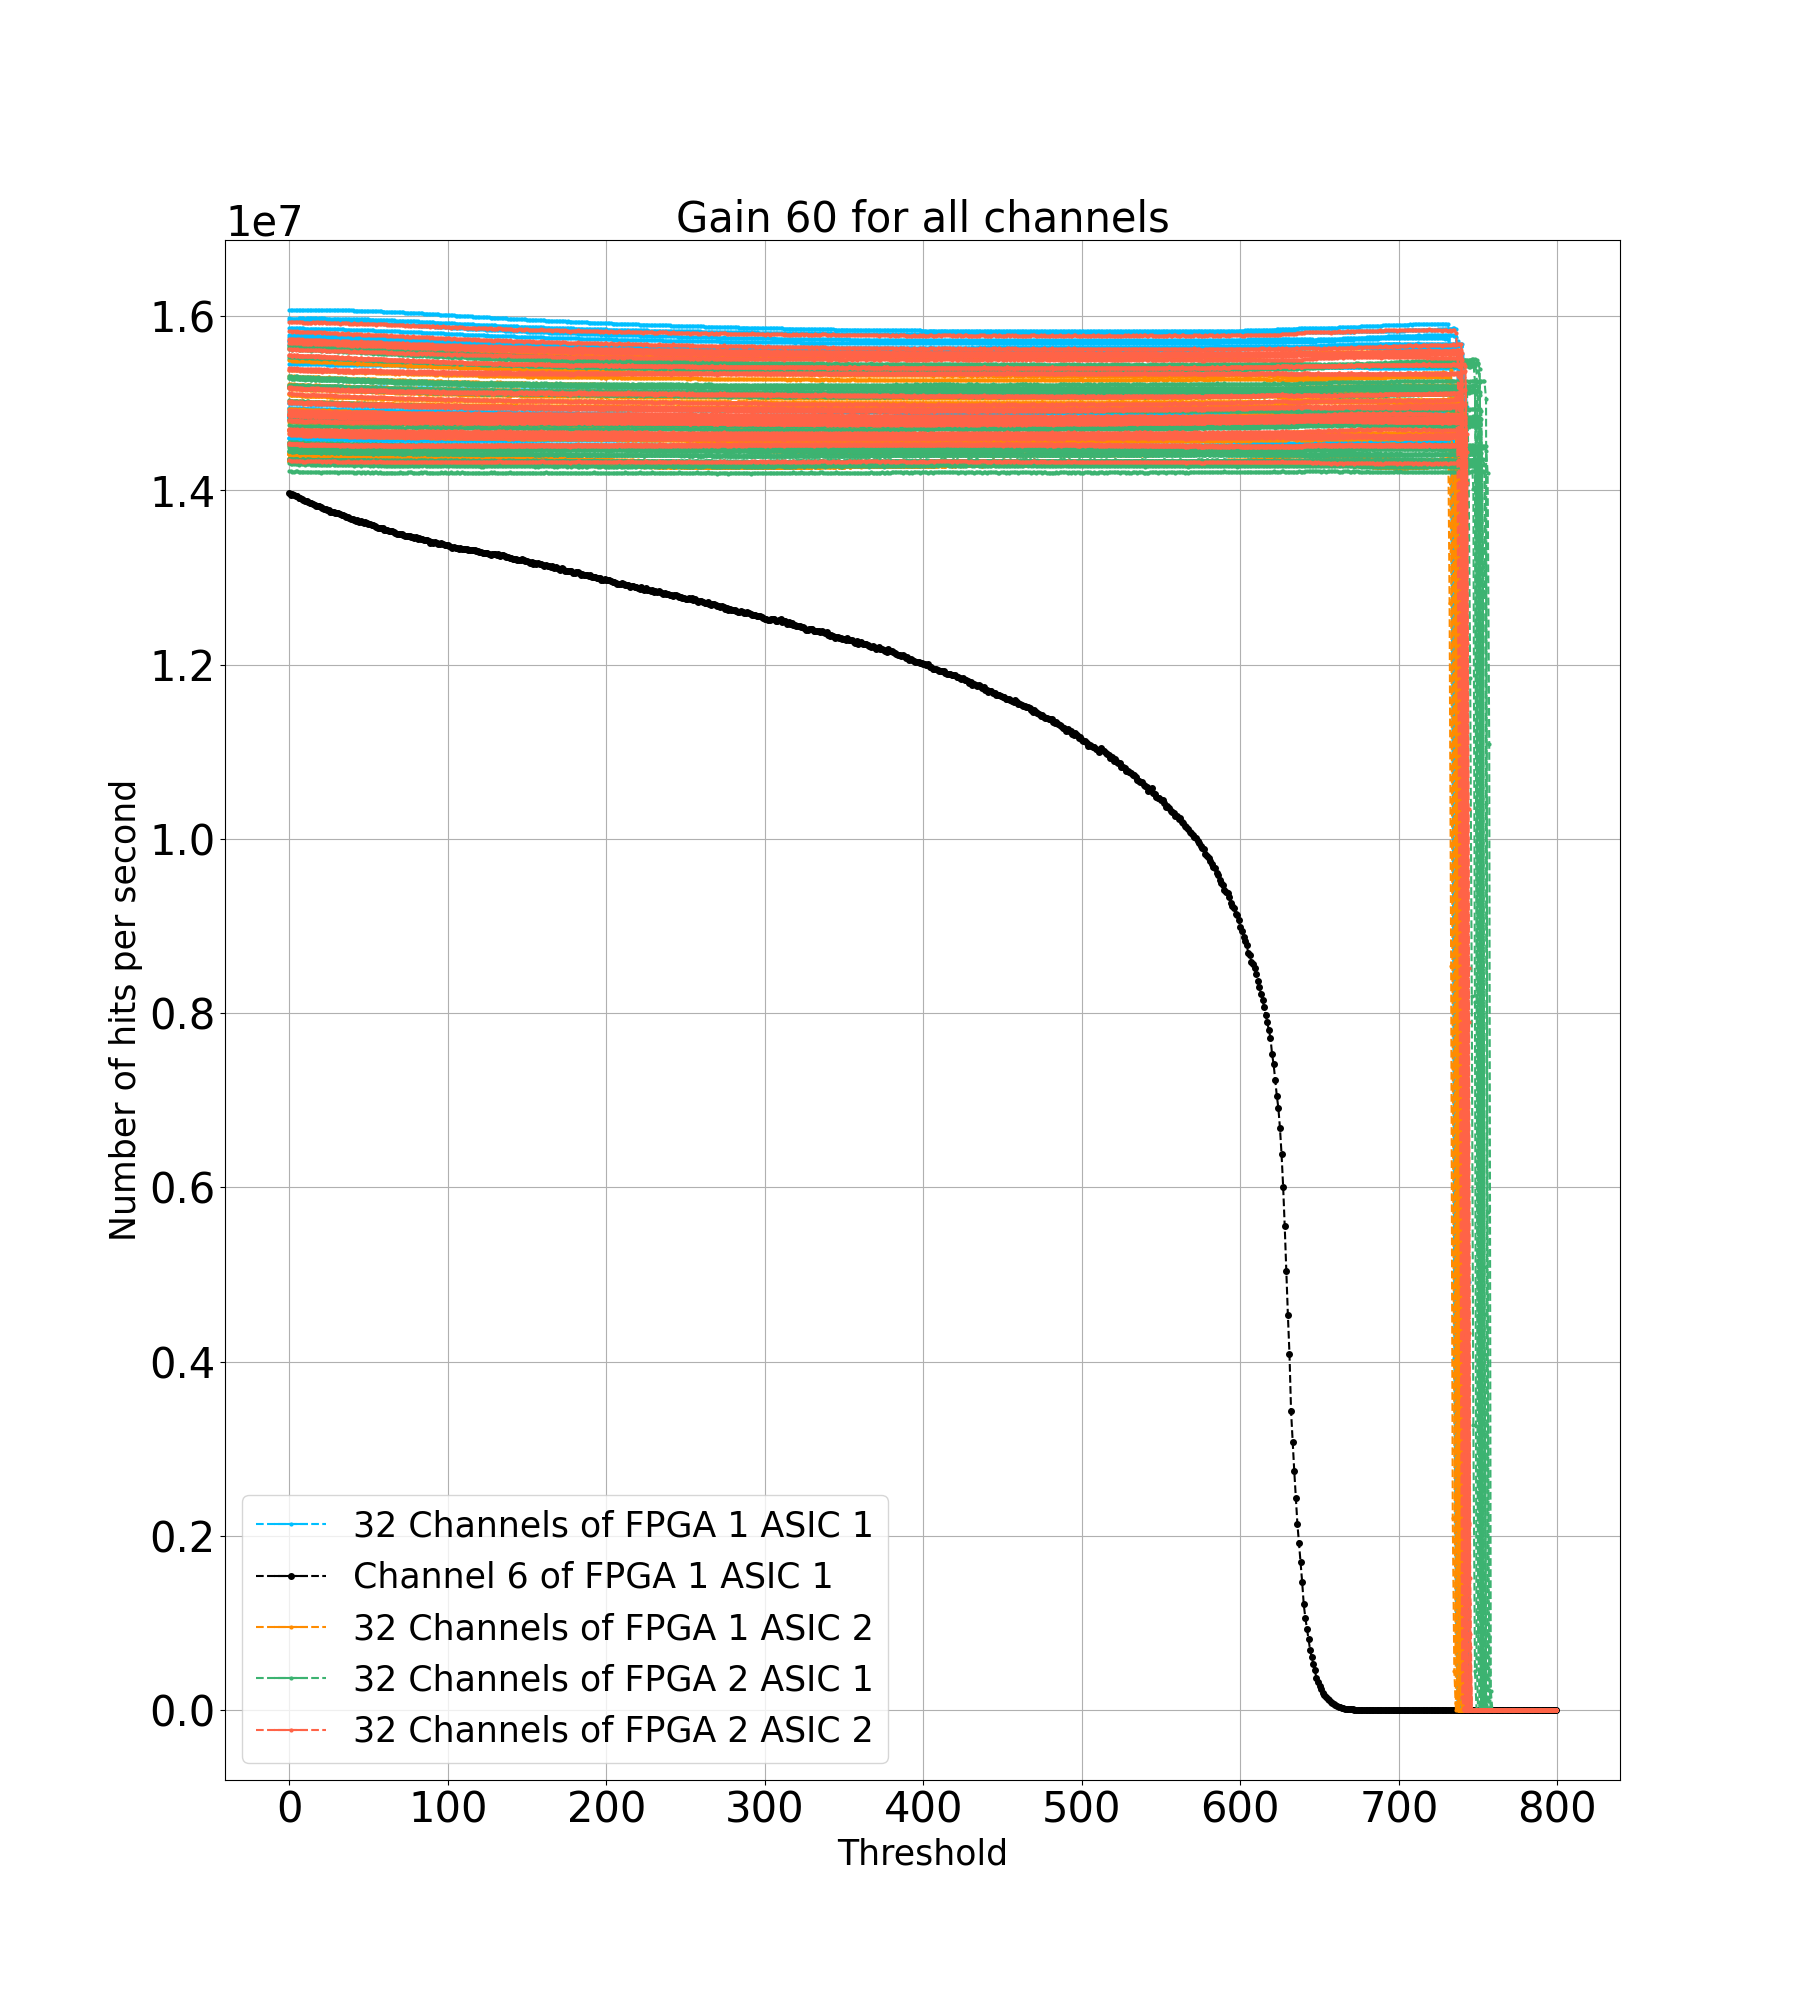
\includegraphics[width=1.0\textwidth]{Gain_60.0_ALLCHANNELS copy.png}
        \caption{Threshold scan of the Citiroc1A ASICs of FPGA 1 and 2 for gain 60 from threshold 0 to 800.}
        \label{fig:threshold_scan_60} 
    \end{figure}
    
    \begin{figure}[H]
        \centering
        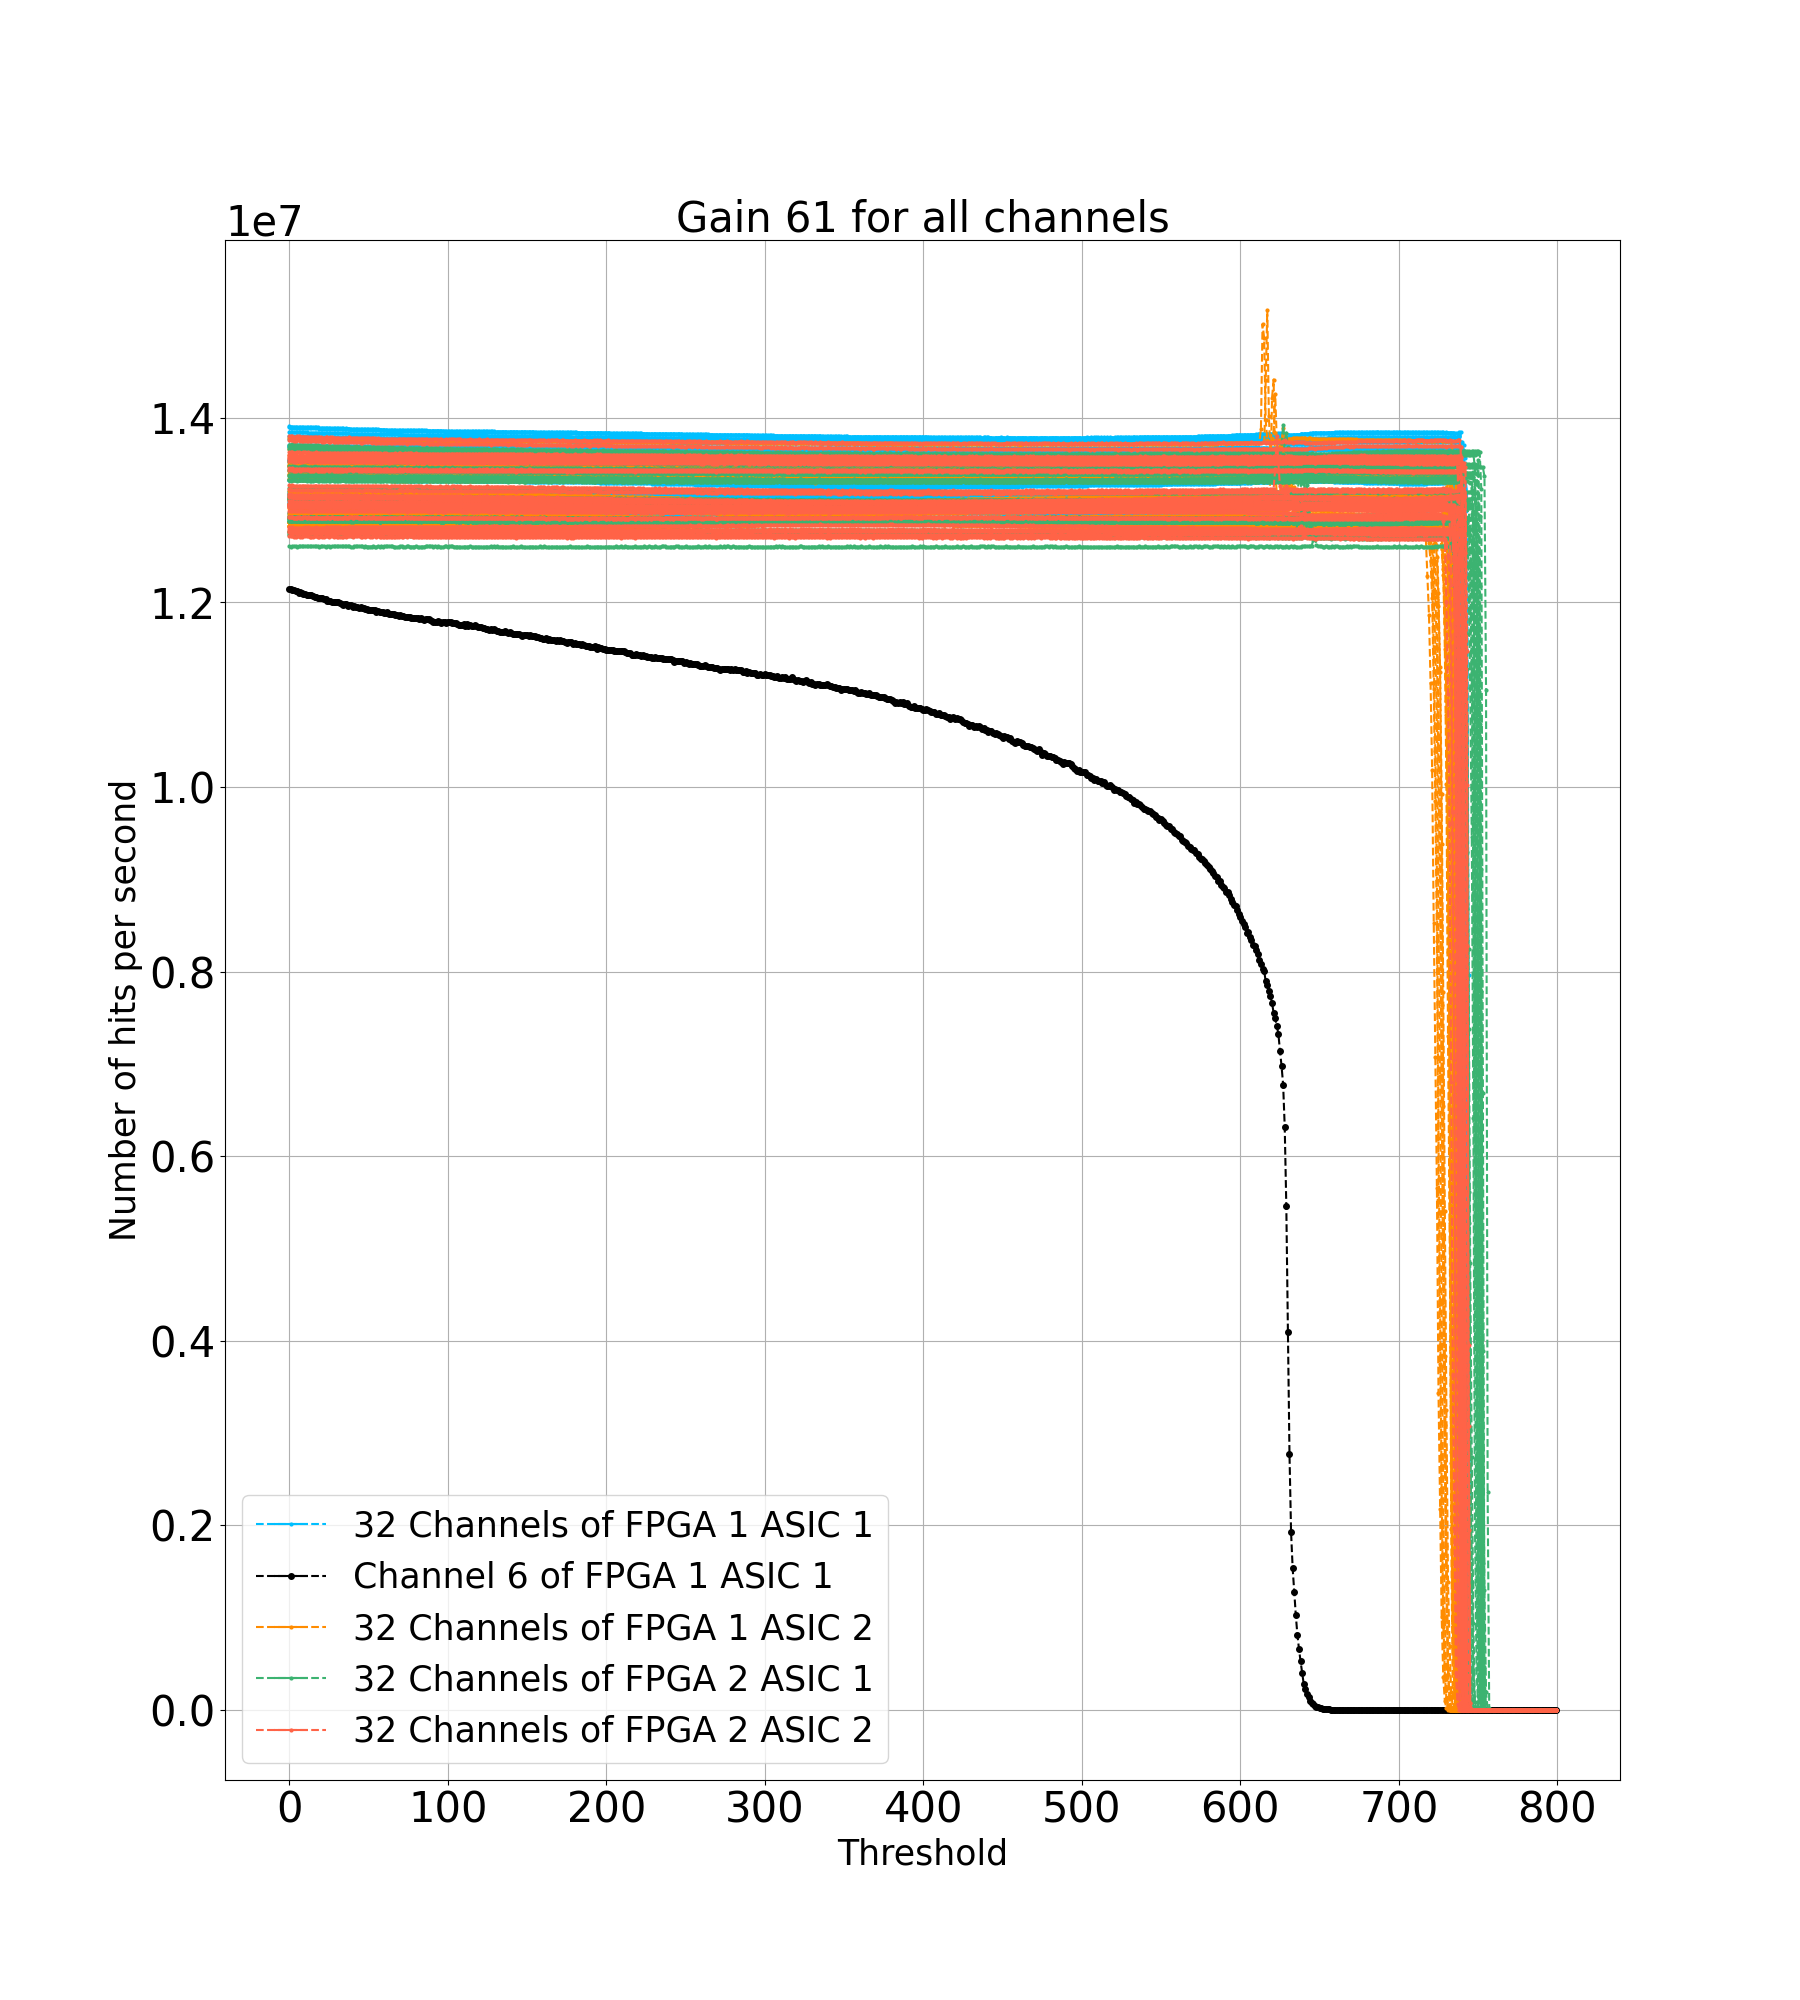
\includegraphics[width=1.0\textwidth]{Gain_61.0_ALLCHANNELS copy 2.png}
        \caption{Threshold scan of the Citiroc1A ASICs of FPGA 1 and 2 for gain 61 from threshold 0 to 800.}
        \label{fig:threshold_scan_61}
    \end{figure}
    
    \begin{figure}[H]
        \centering
        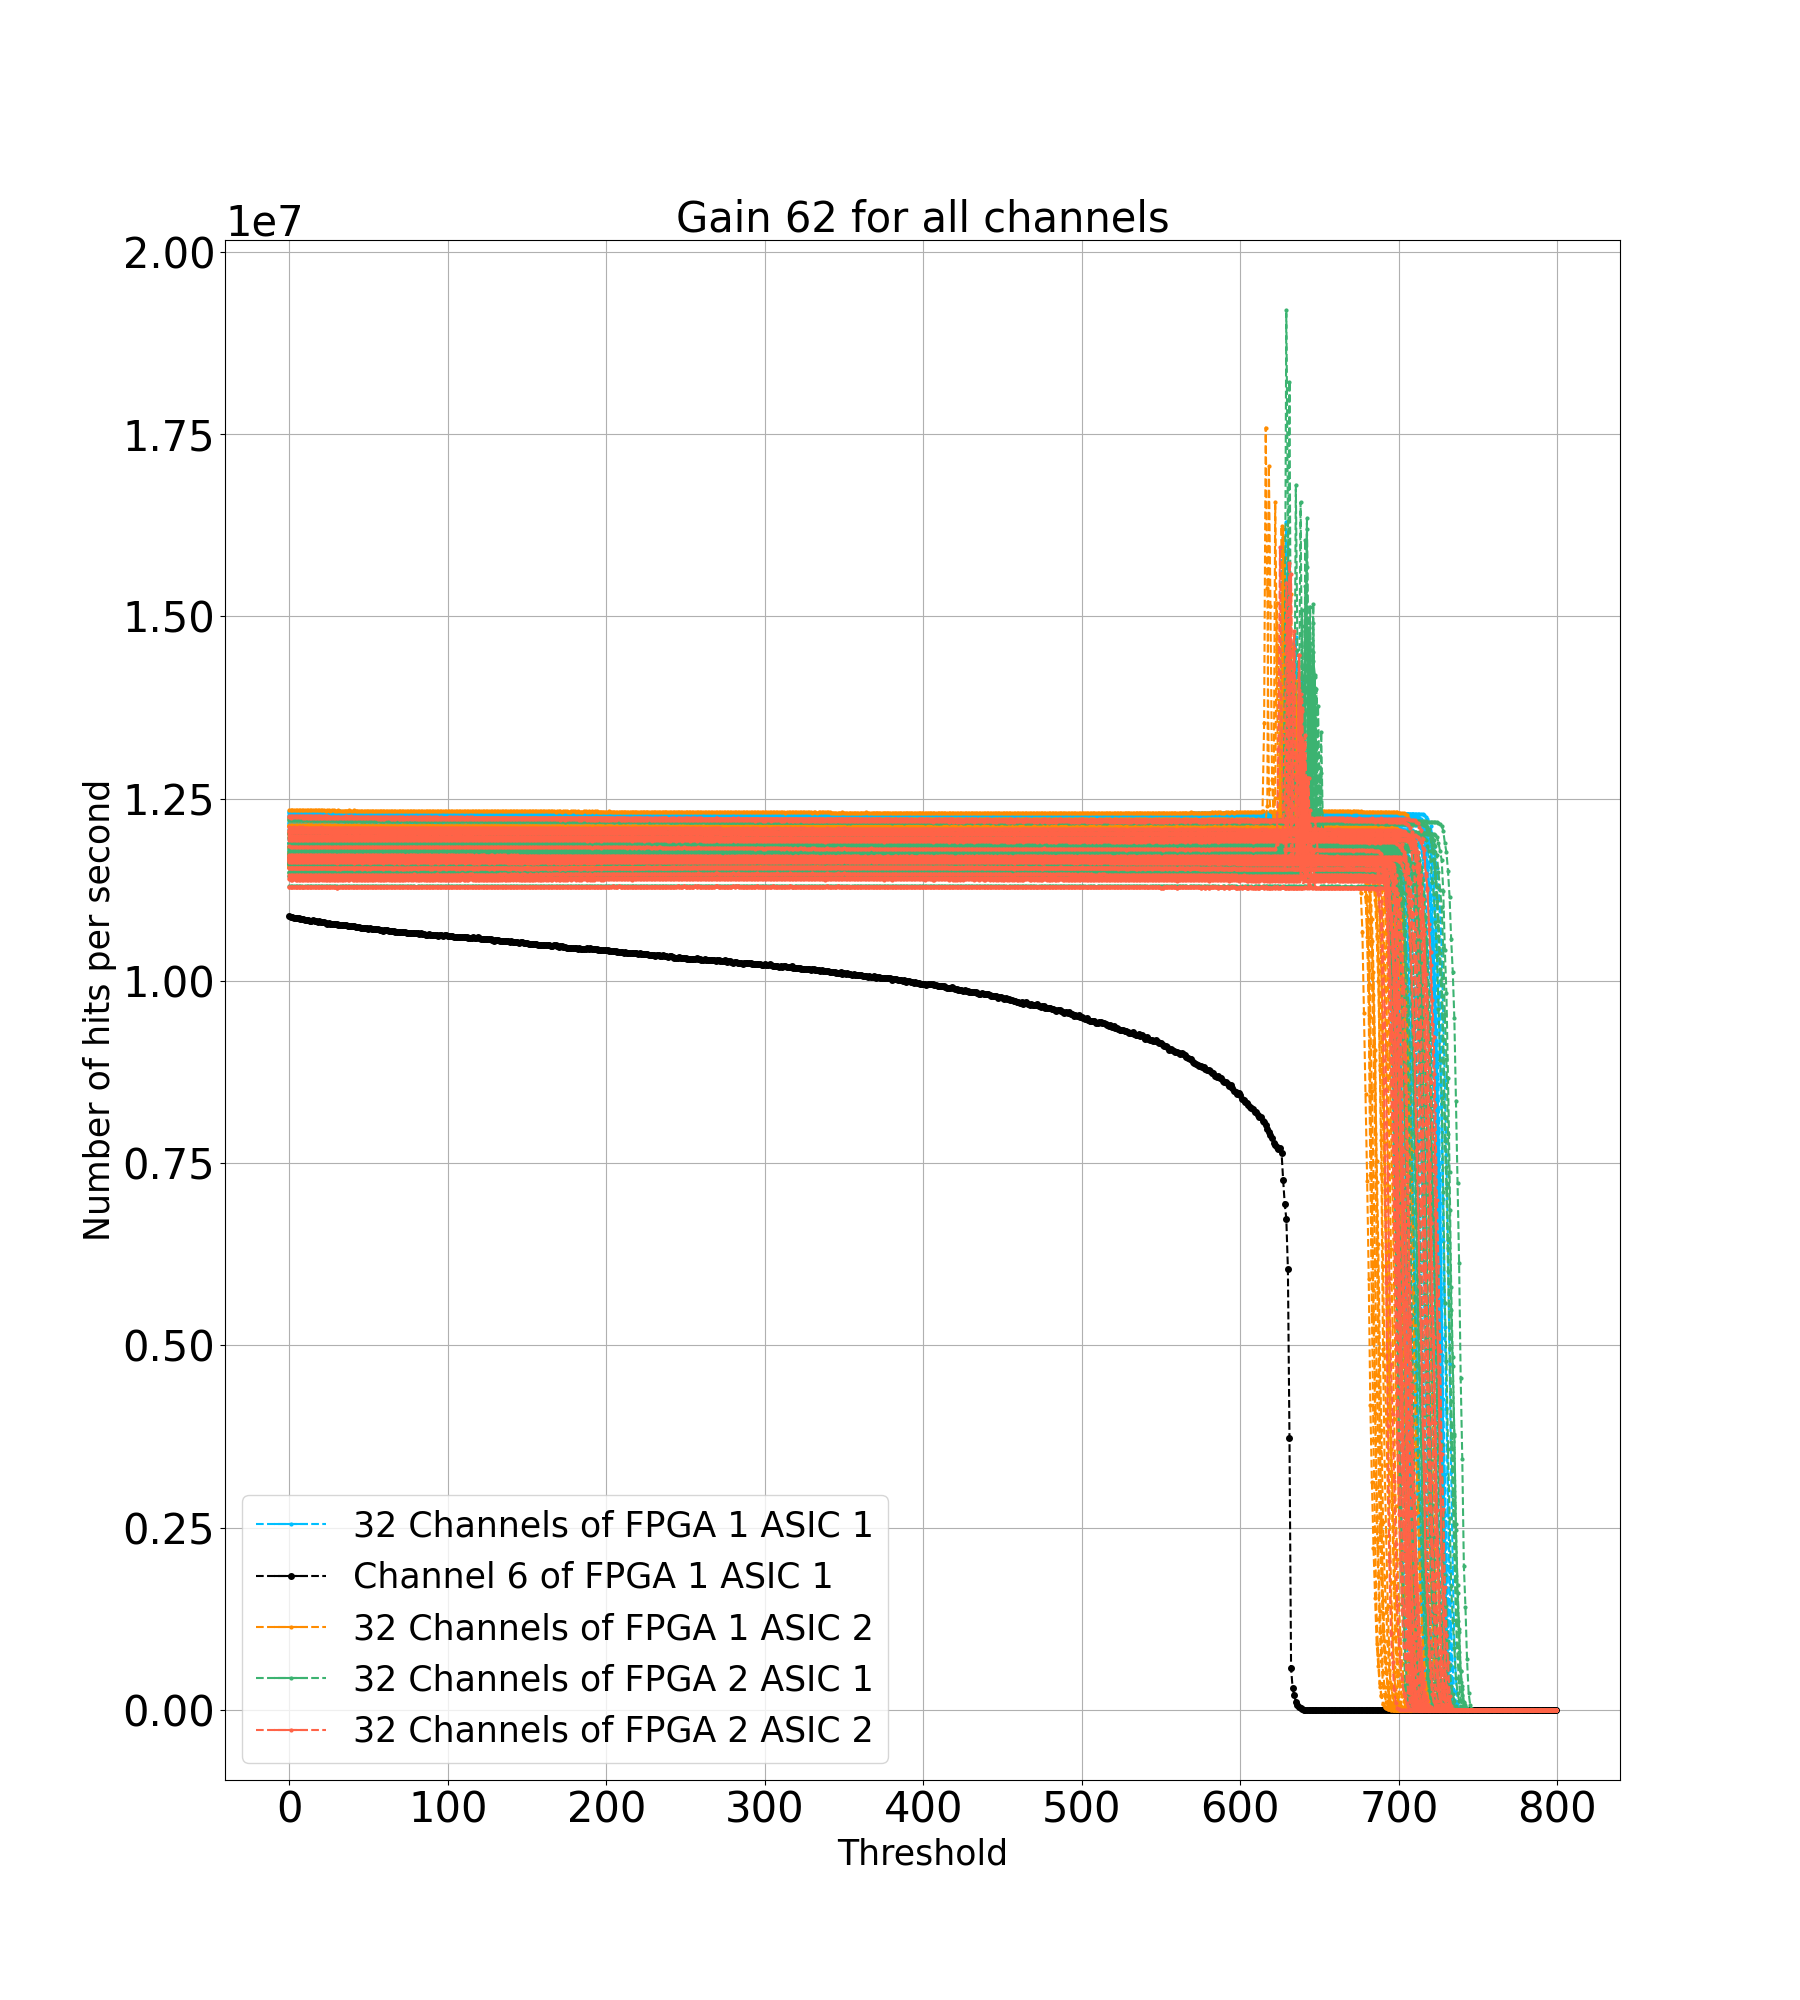
\includegraphics[width=1.0\textwidth]{Gain_62.0_ALLCHANNELS copy 2.png}
        \caption{Threshold scan of the Citiroc1A ASICs of FPGA 1 and 2 for gain 62 from threshold 0 to 800.}
        \label{fig:threshold_scan_62}
    \end{figure}
    \section{Frontend Electronics Characterization}
    \subsection{Firmware Evaluation}
    Before performing the final noise measurements, I thoroughly verified the firmware functionality by performing the following tests:
    \begin{itemize}
        \item Using the internal probing capabilities of the Citiroc1A to verify the configuration of the ASICs, described in section~\ref{sec:probe_register}.
        \item Turning off individual channels of the ASICs by turning off the amplification of the channels or setting it to a low gain.
        \item Disabling specific stages of the ASIC, such as the fast shaper or the time discriminator.
        \item Using the output configuration of the Citiroc1A to turn off all triggers of the ASICs.
    \end{itemize}
    \subsection{S-curve Analysis}
    In order to determine the optimal threshold and characterize the noise of the ASICs of FPGA 1 and 2, an S-curve analysis was performed.
    \newline
    The falling edge of the pedestal is fitted with the S-curve described in section~\ref{sec:noise_theory}
    \newline
    The results of the S-curve analysis are shown exemplarily for channel 0 of Citiroc1A 1 of FPGA 1 with gain 60,61 and 62 in Figs.~\ref{fig:S_curve_60},~\ref{fig:S_curve_61} and~\ref{fig:S_curve_62}.
    
    \begin{figure}[H]
        \centering
        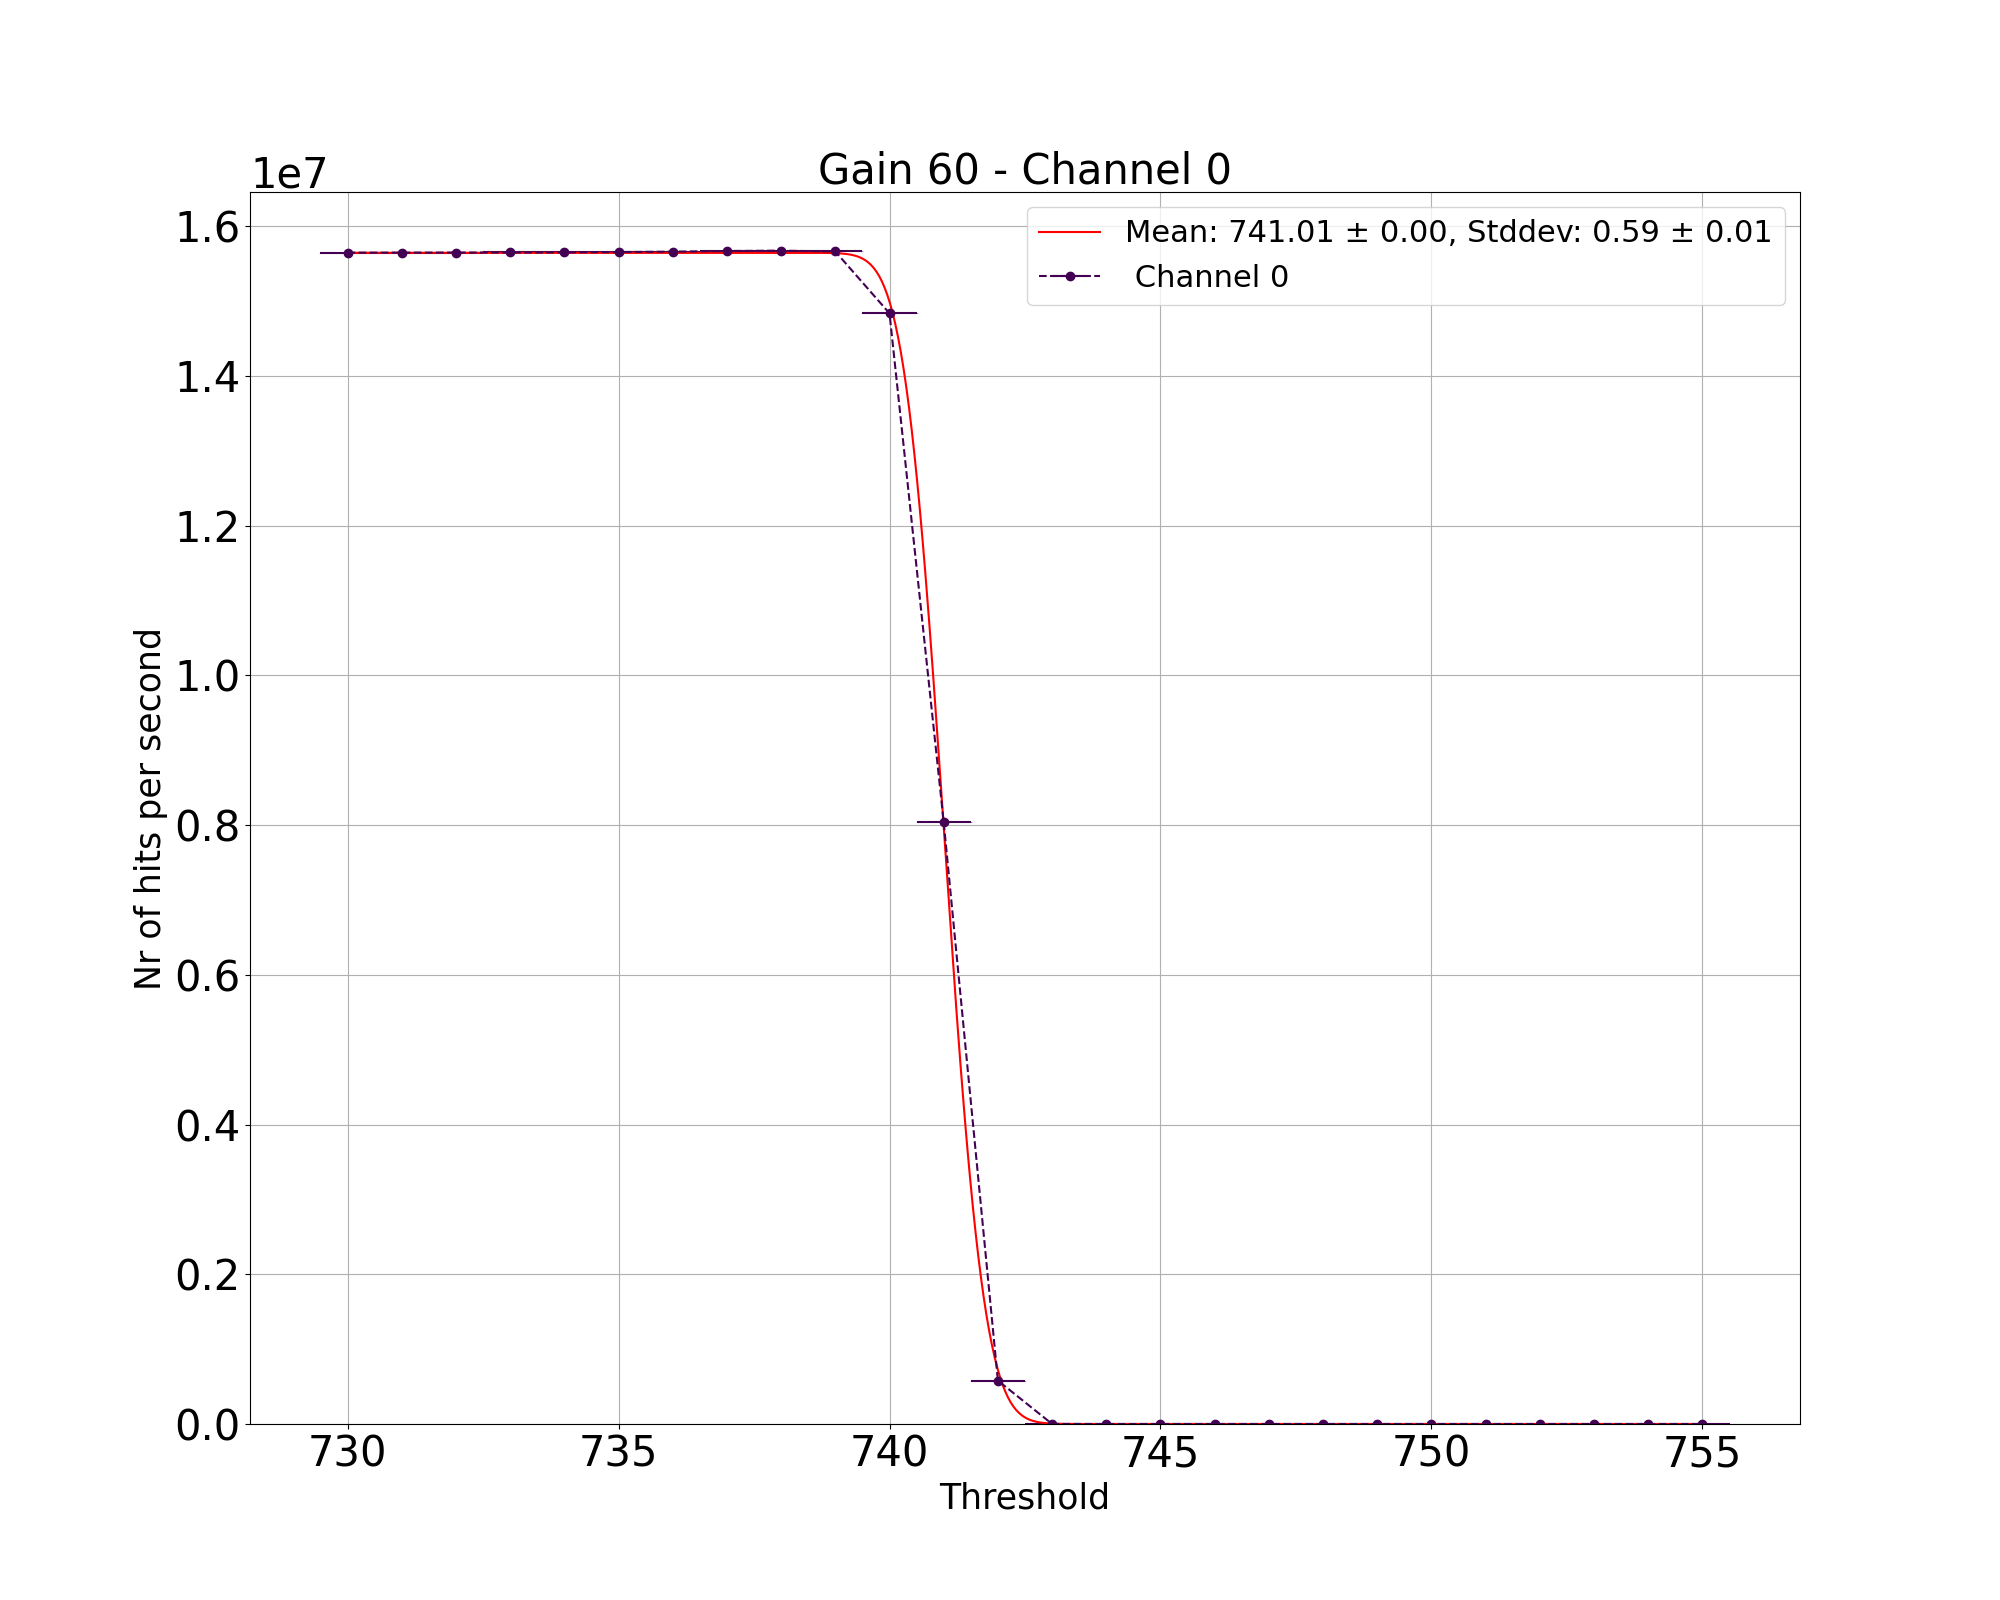
\includegraphics[width=0.7\textwidth]{Runs_170_400_Gain_60.0_0_ChannelALL_FPGAS copy 3.png}
        \caption{Results of the S-curve analysis for channel 0 of Citiroc1A 1 of FPGA 1 with gain 60.}
        \label{fig:S_curve_60}
    \end{figure}
    \begin{figure}[H]
        \centering
        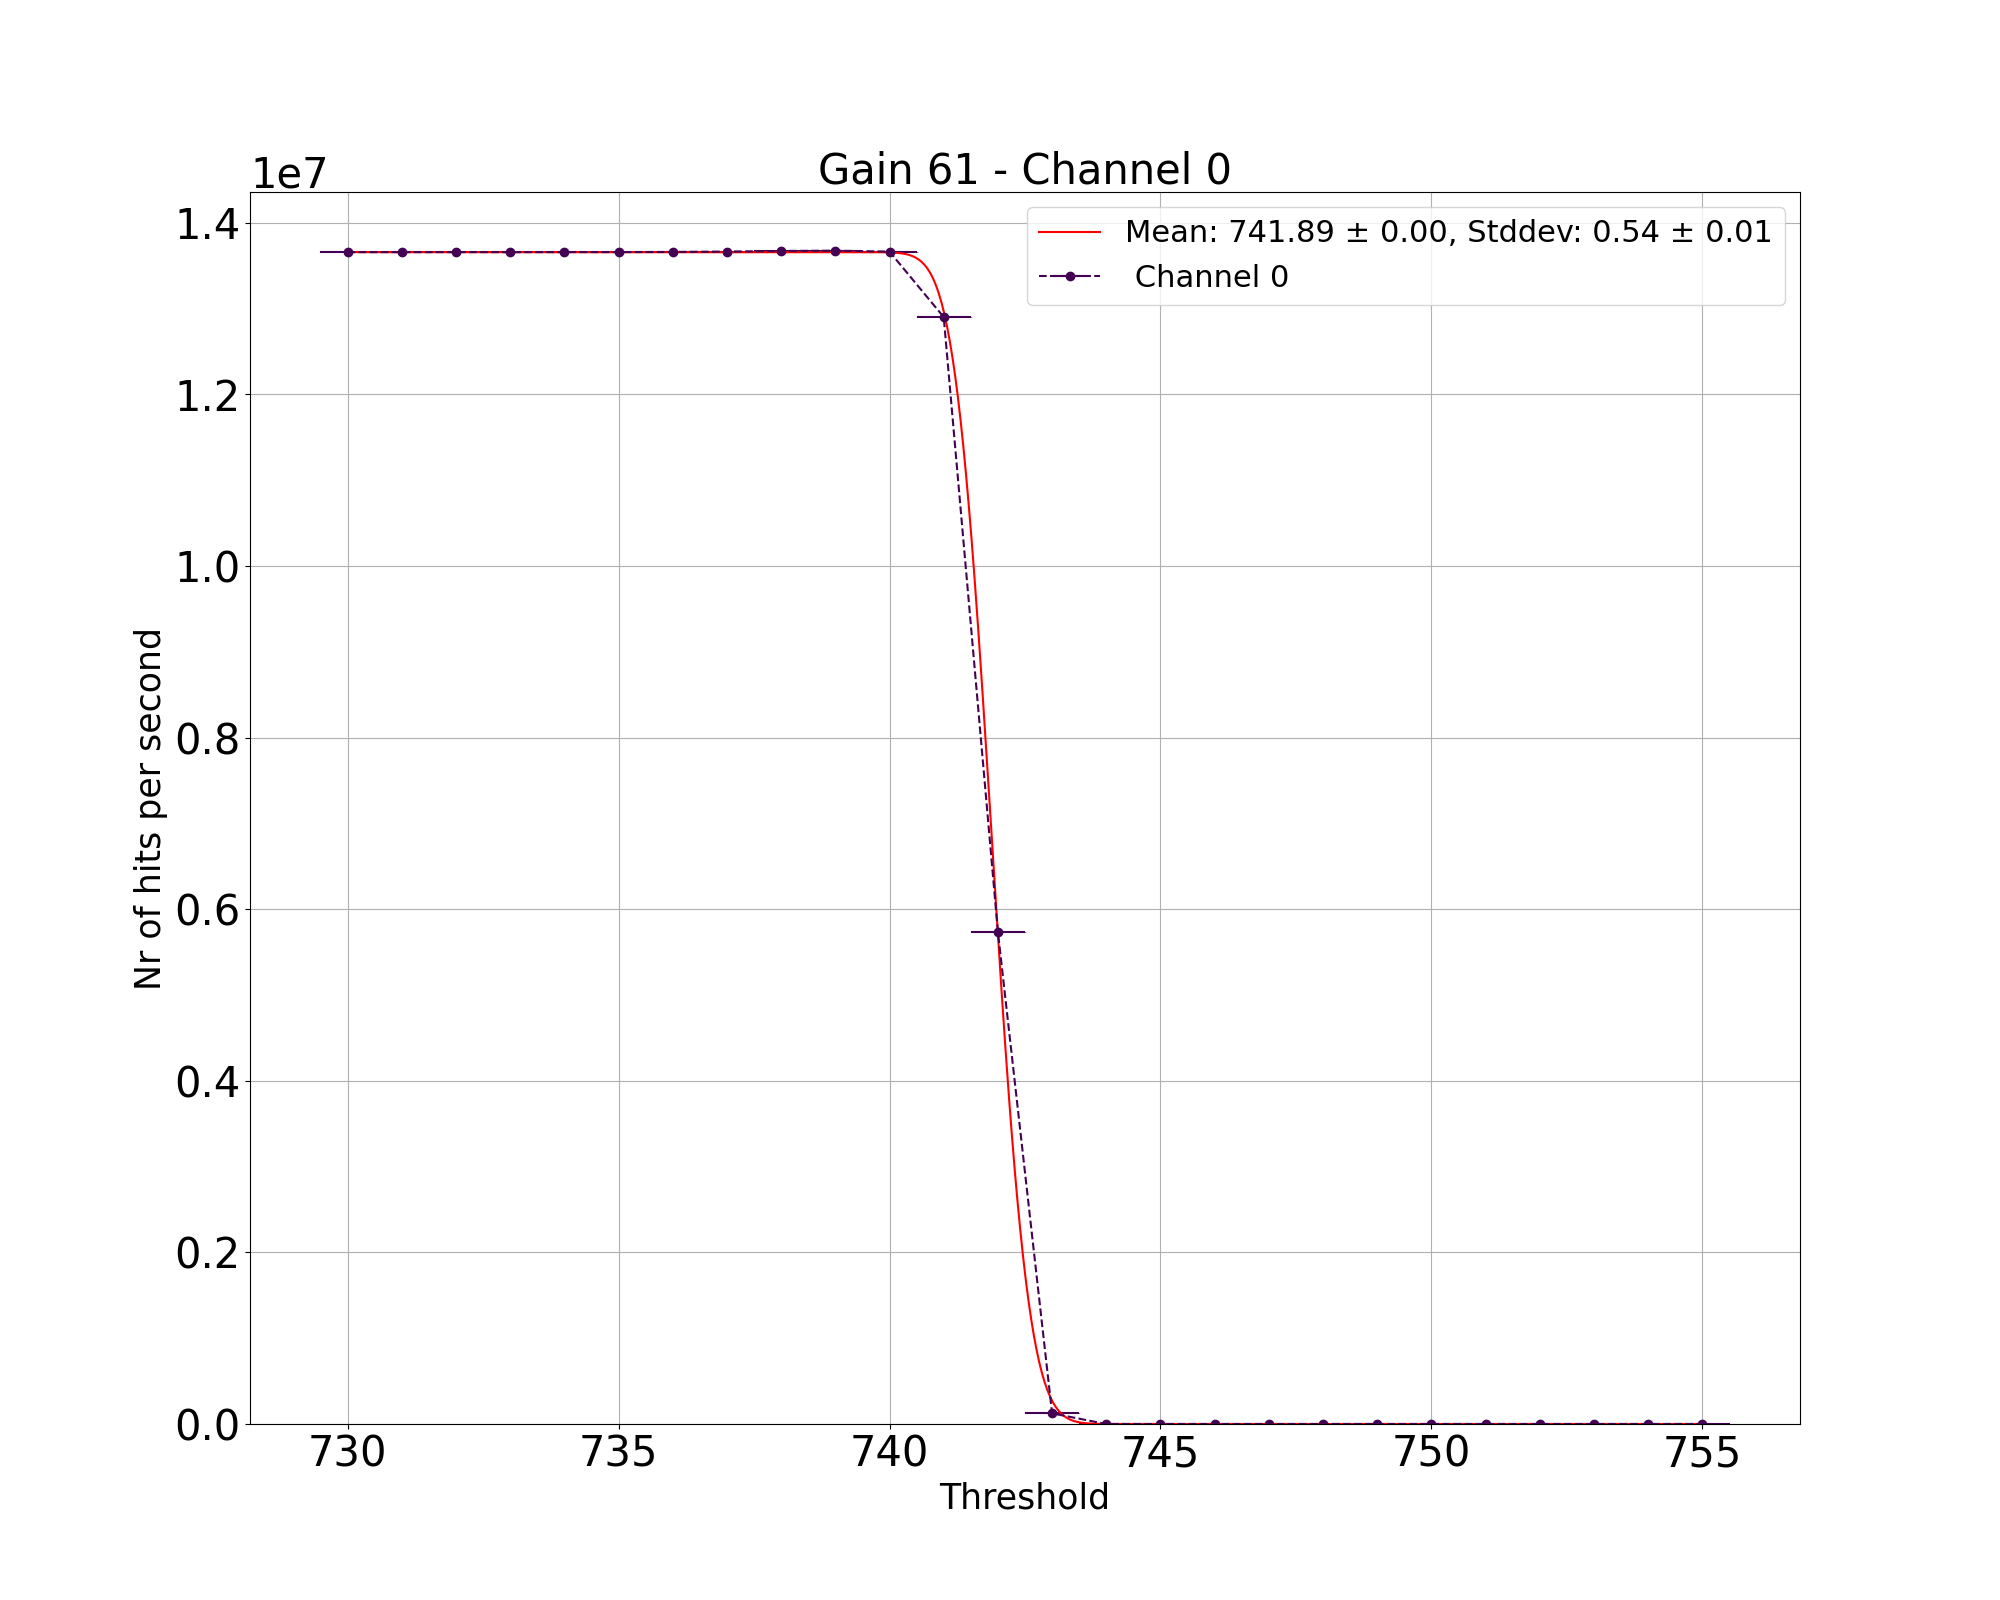
\includegraphics[width=0.7\textwidth]{Runs_170_400_Gain_61.0_0_ChannelALL_FPGAS copy 3.png}
        \caption{Results of the S-curve analysis for channel 0 of Citiroc1A 1 of FPGA 1 with gain 61.}
        \label{fig:S_curve_61}
    \end{figure}
    \begin{figure}[H]
        \centering
        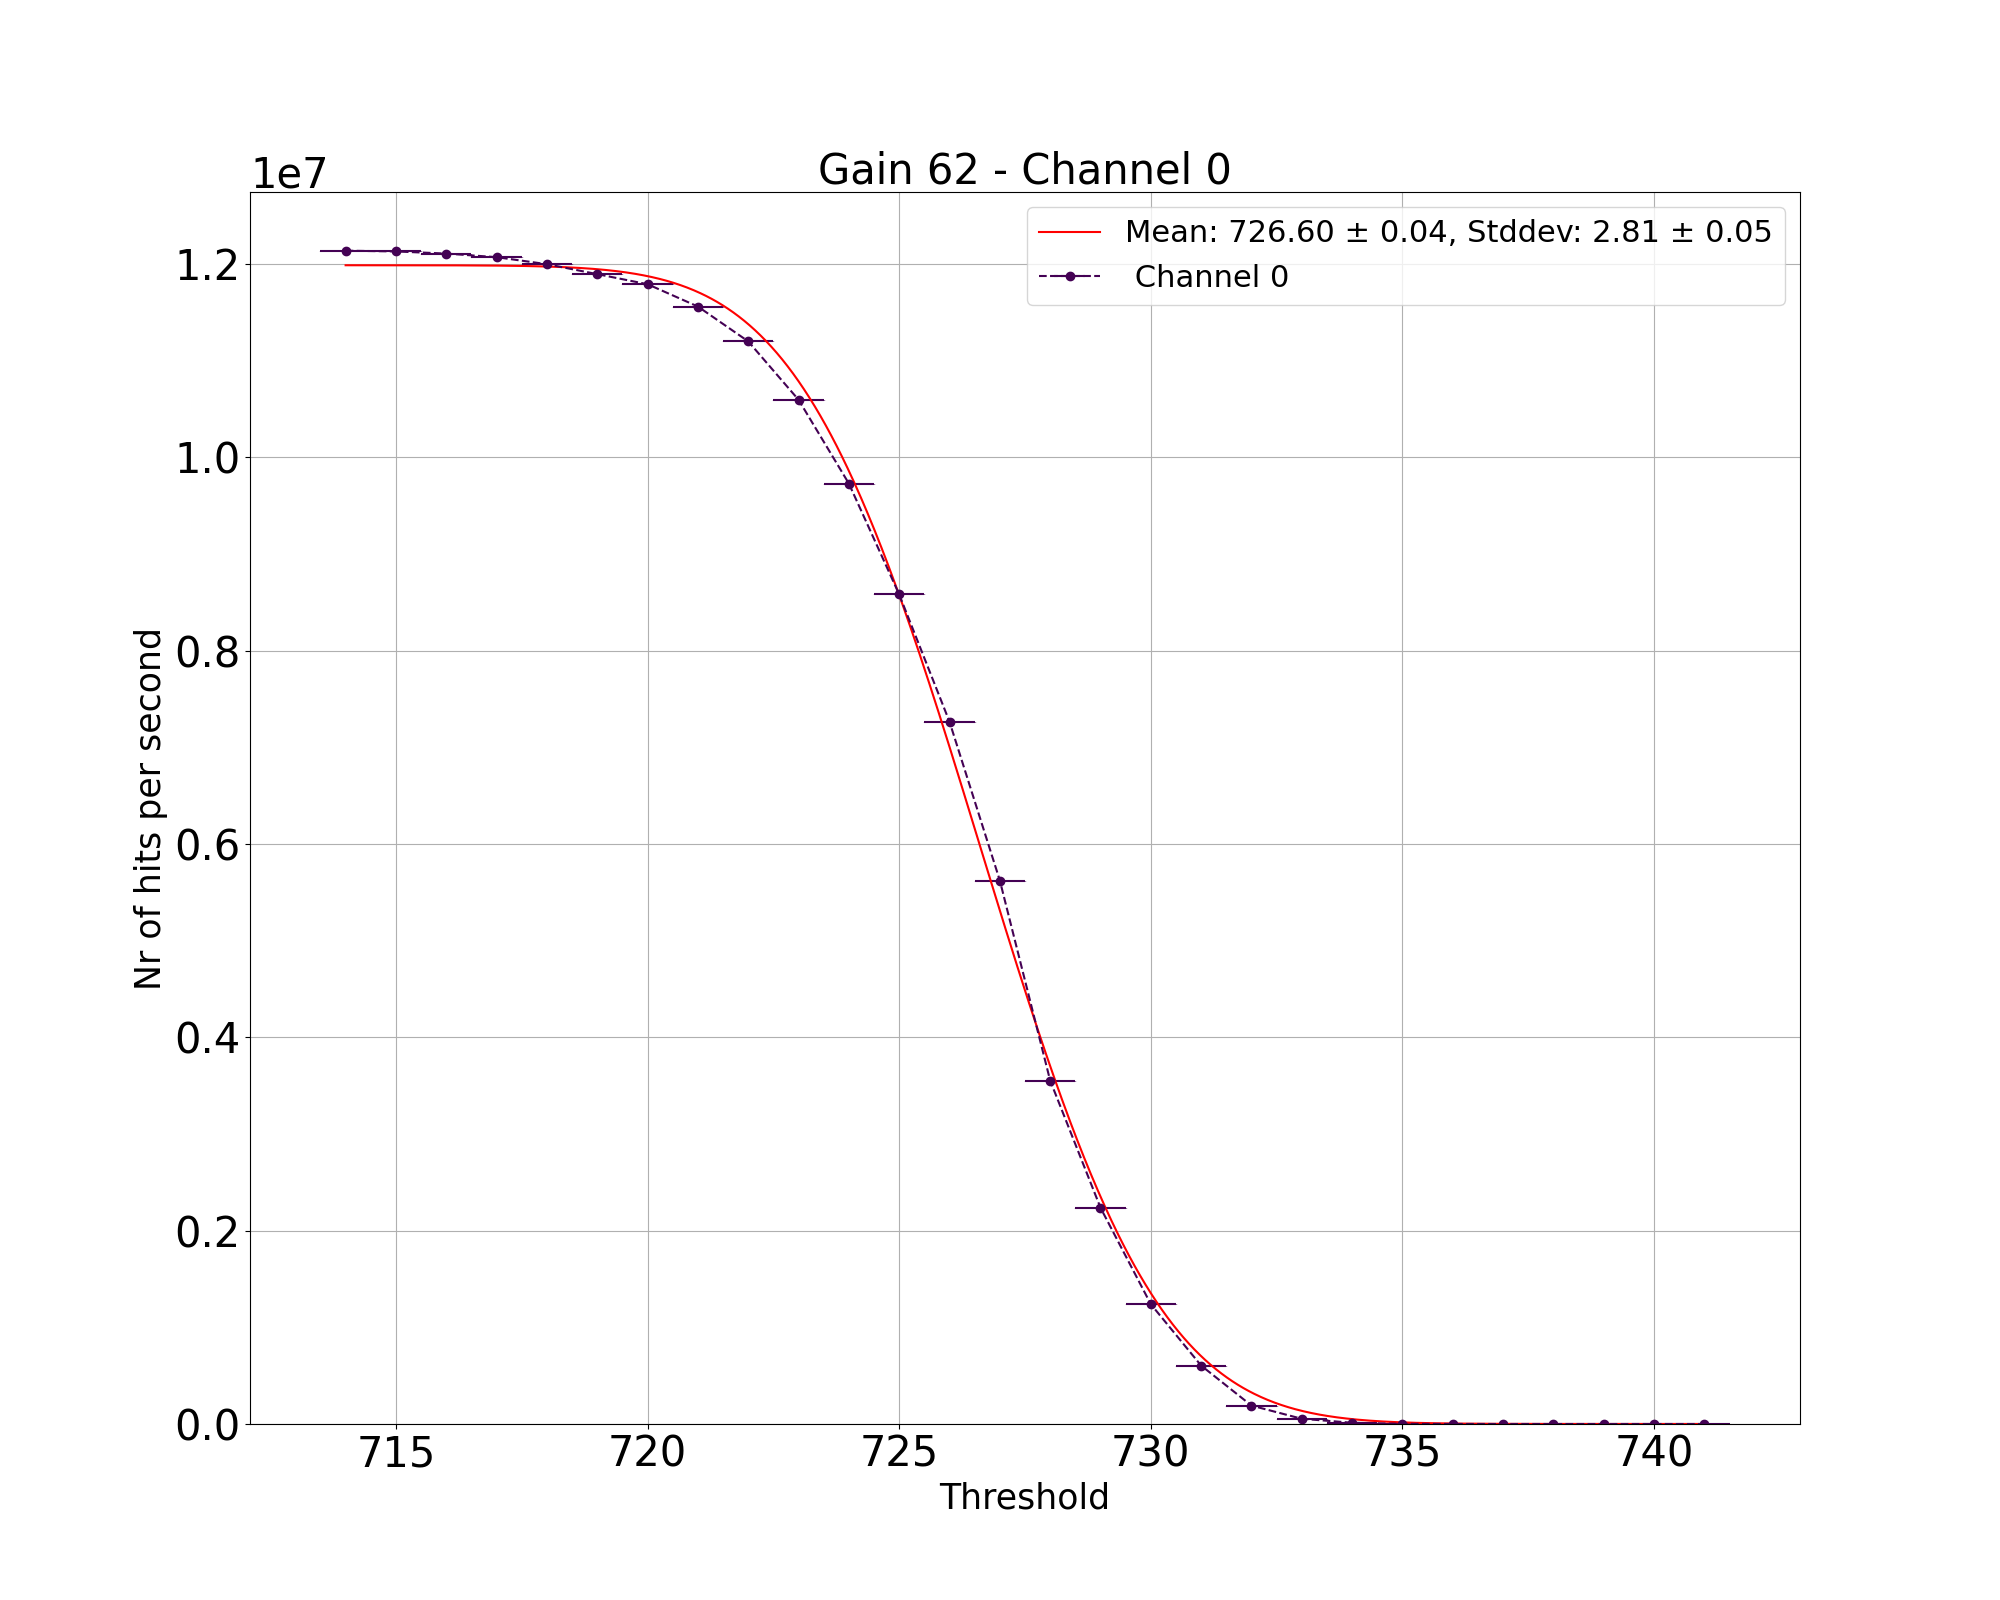
\includegraphics[width=0.7\textwidth]{Runs_170_400_Gain_62.0_0_ChannelALL_FPGAS copy 3.png}
        \caption{Results of the S-curve analysis for channel 0 of Citiroc1A 1 of FPGA 1 with gain 62.}
        \label{fig:S_curve_62}
    \end{figure}
    The S-curve fit, for all channels, for the high gain of 62 needed for the PRM experiment is shown in Fig.~\ref{fig:S_curve_62_ALL}. 
    
    \begin{figure}[H]
        \centering
        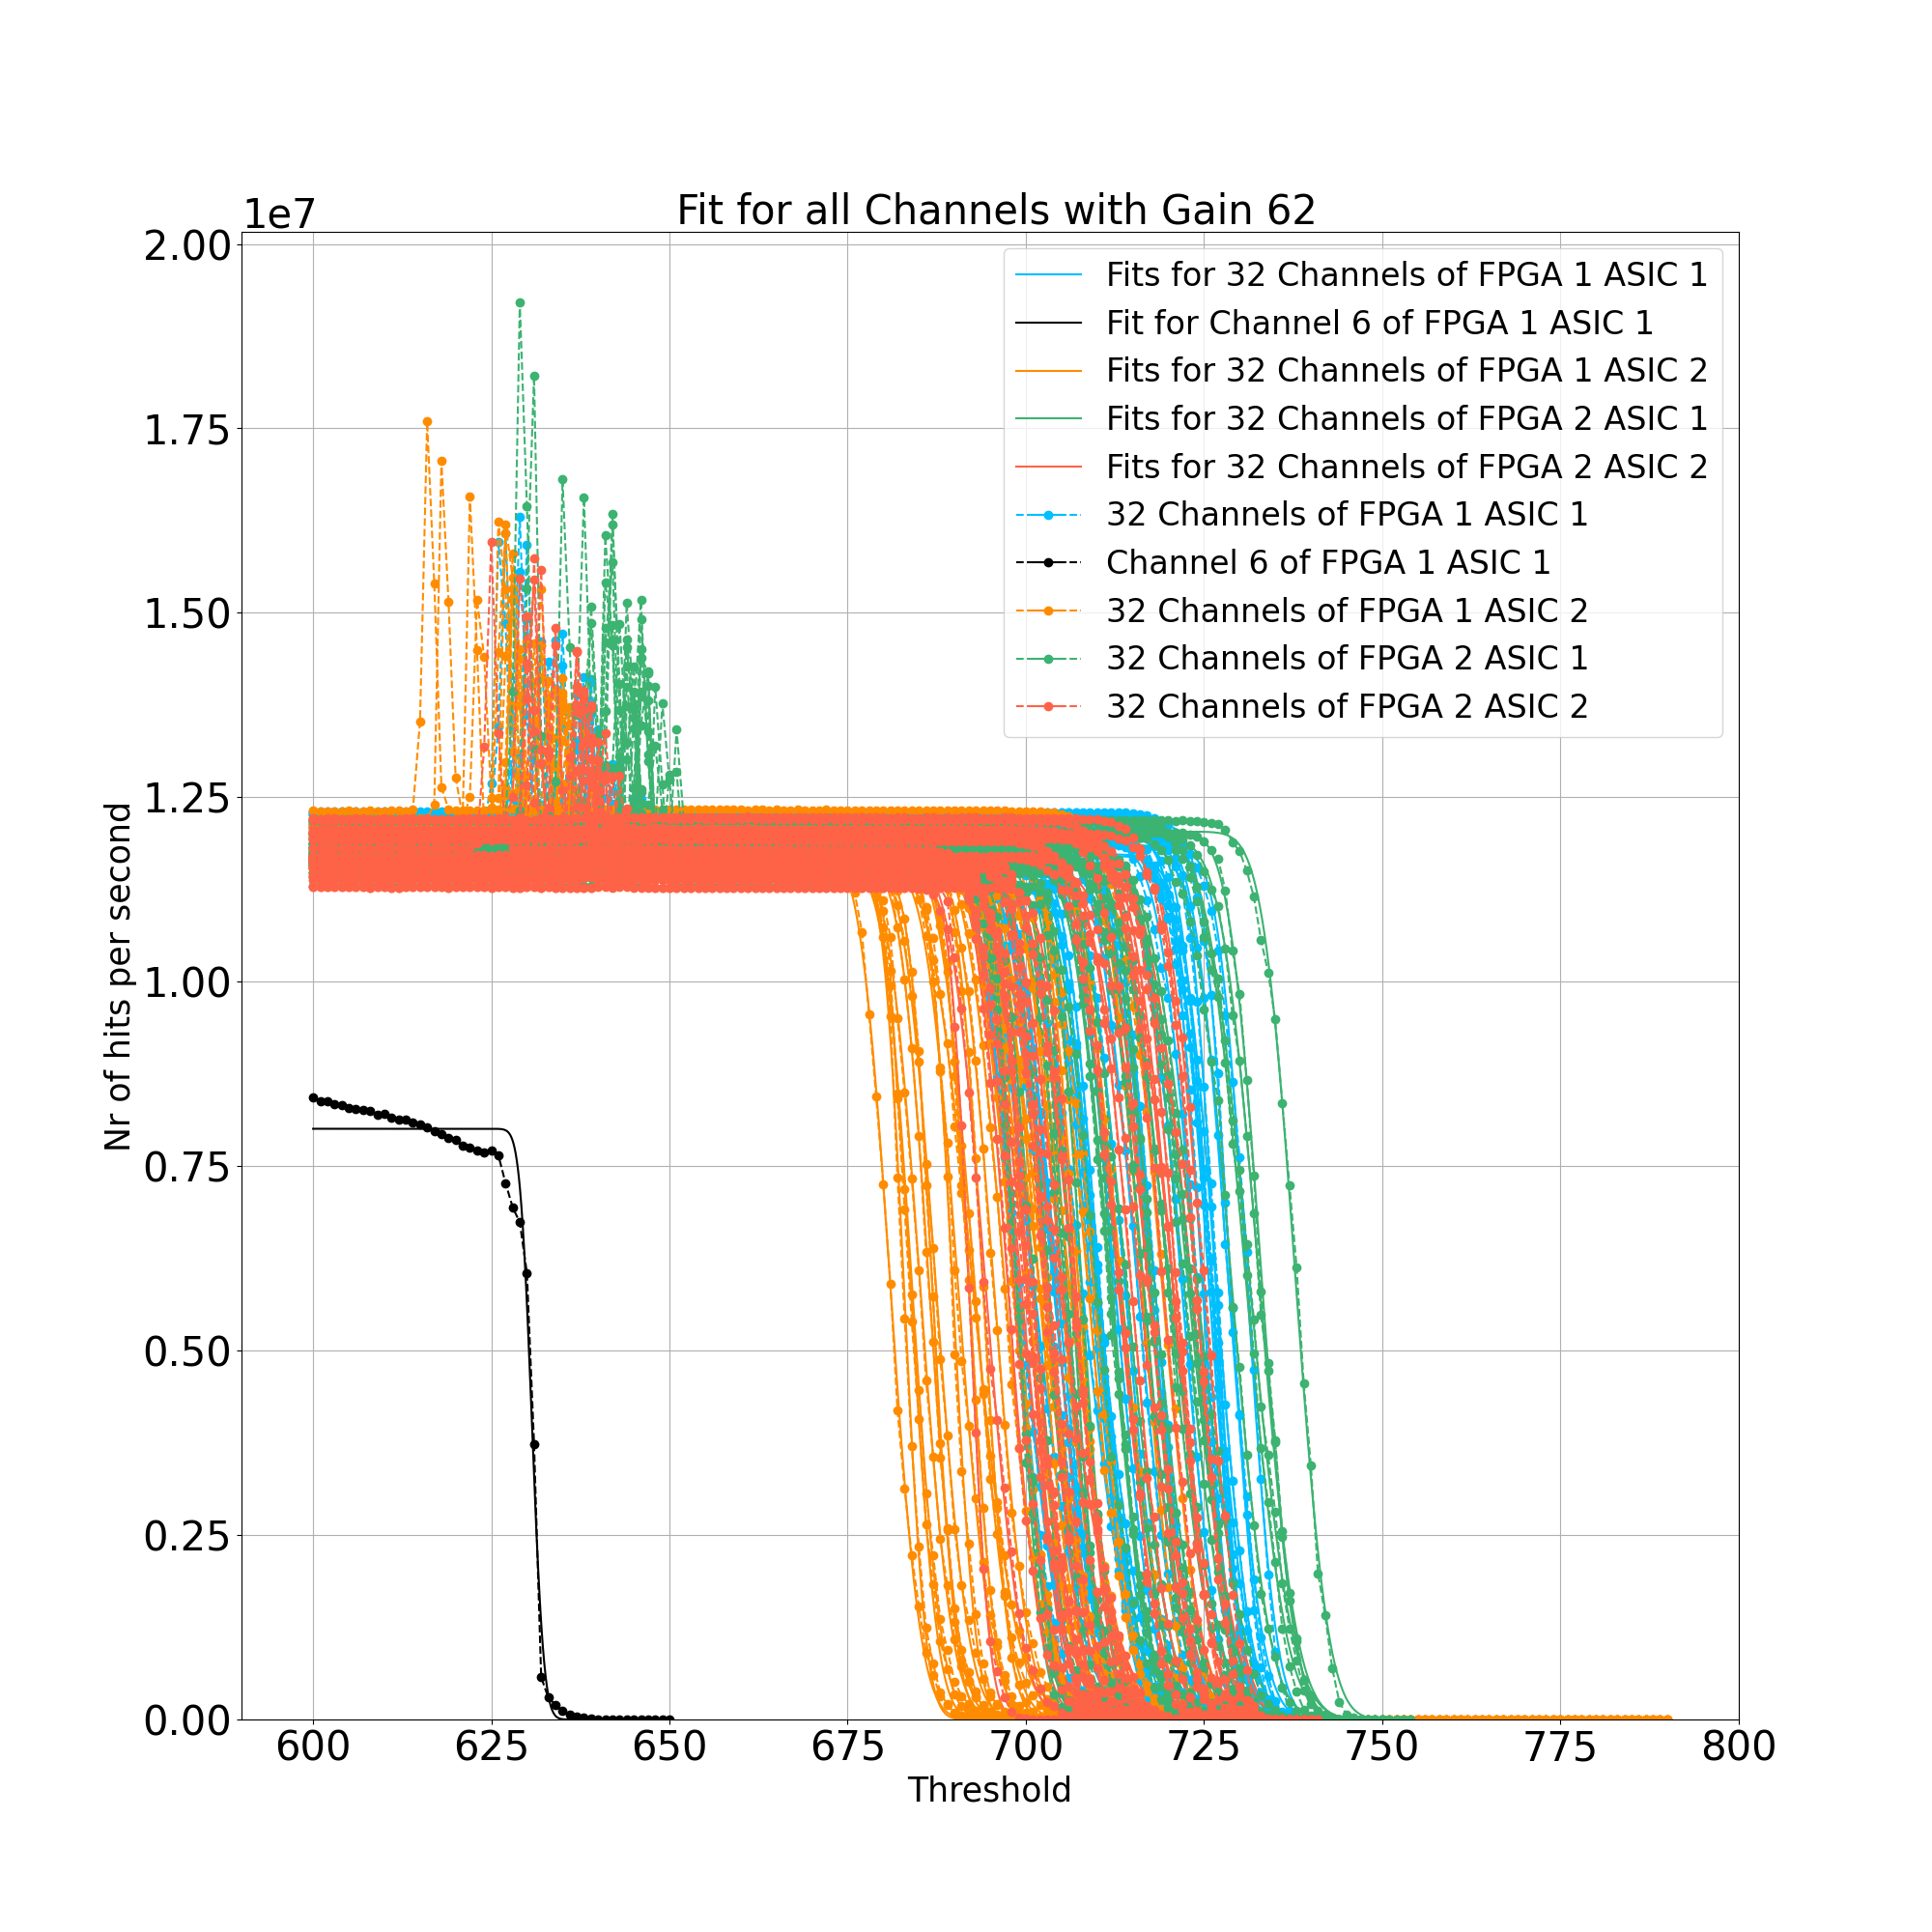
\includegraphics[width=1.0\textwidth]{Fit for all Channels with Gain 62 copy 5.png}
        \caption{Results of the S-curve analysis for all channels of the Citiroc1A ASICs of FPGA 1 and 2 with gain 62.}
        \label{fig:S_curve_62_ALL}
    \end{figure}
    The mean $\mu$ and the standard deviation $\sigma$ of the noise distribution were determined from the S-curve fits and are shown in Appendix \ref{cha:appendixFitPar}.
    They are plotted against the gain for all channels in Figure \ref{fig:Mean vs gain}.
    \begin{figure}[H]
        \centering
        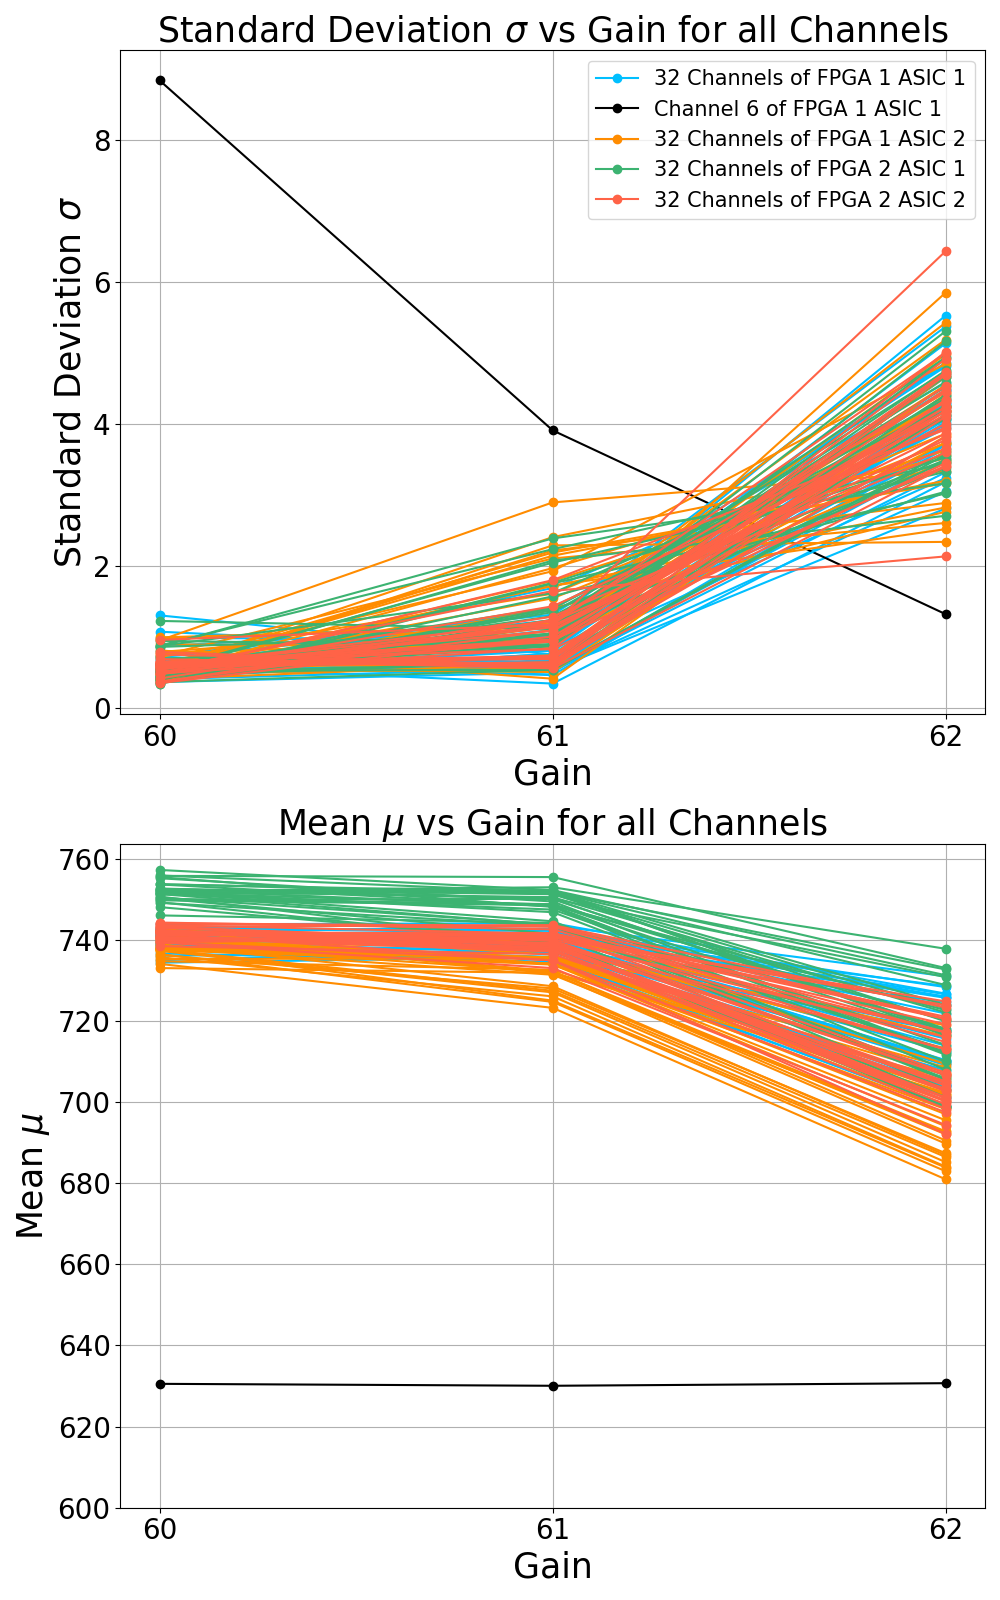
\includegraphics[width=0.7\textwidth]{Individual_Stddev_and_Mean_vs_Gain copy 4.png}
        \caption{Mean $\mu$ and standard deviation $\sigma$ determined from the S-curve fits for all channels of the Citiroc1A ASICs of FPGA 1 and 2 plotted vs the gain.}
        \label{fig:Mean vs gain}
    \end{figure}
    
    \subsection{Comparison with Evaluation Board} 
    A comparison of the threshold scan to one performed with the same configuration of the Citiroc1A ASIC on a by Weeroc company provided Evaluation Board with gain 58 is shown in Fig.~\ref{fig:threshold_scan_comparison_58}.% and 62 is shown in Figures \ref{fig:threshold_scan_comparison_58} and \ref{fig:threshold_scan_comparison_62}. 
    \begin{figure}[H]
        \centering
        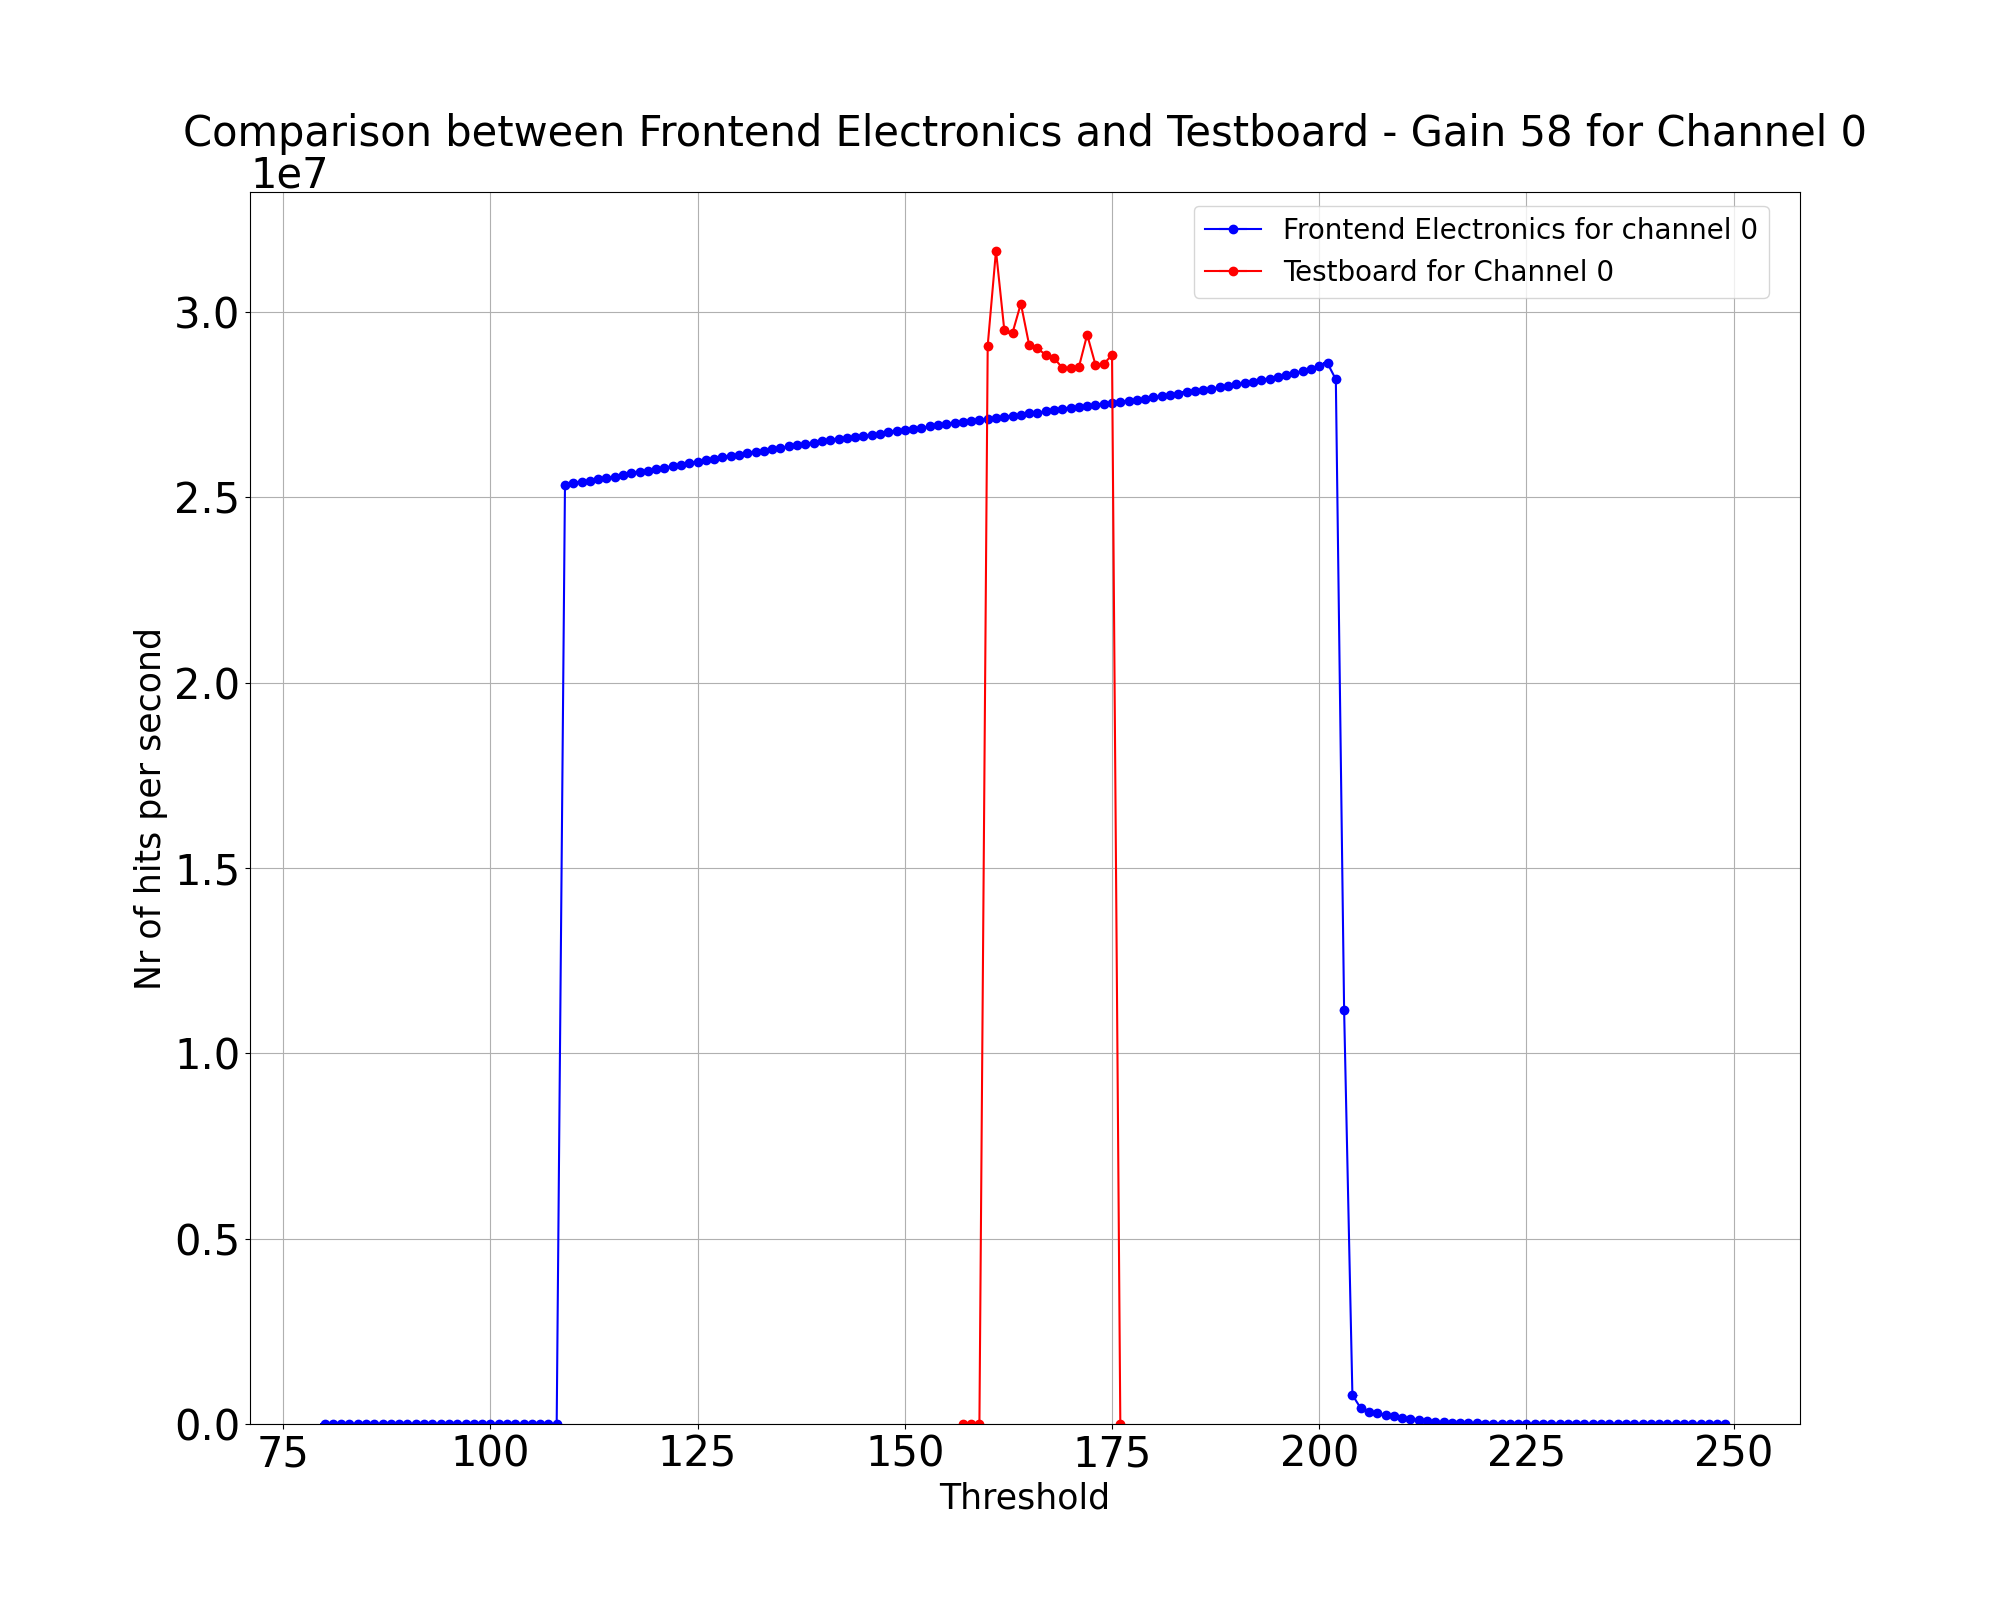
\includegraphics[width=1.0\textwidth]{Runs_170_400_Gain_58.0_0_Channel_compare copy 2.png}
        \caption{Comparison of the threshold scan of the frontend electronics to the threshold scan performed on a by Weeroc company provided Evaluation Board with a gain of 58.}
        \label{fig:threshold_scan_comparison_58}
    \end{figure}
    
 
    The pedestal of the threshold scan performed with the frontend electronics is far larger than the pedestal of the threshold scan performed with the Evaluation Board.
    This difference in the observed behaviour of the frontend electronics can currently not be explained.
    \subsection{Behaviour at different Gain Setting}
    The threshold scan of the Citiroc1A ASICs in the frontend electronics shows different behaviour for gain ranges of 0 to 58 (Figs.~\ref{fig:threshold_scan_58}) and 60 to 62 (Figs.~\ref{fig:threshold_scan_60},~\ref{fig:threshold_scan_61} and~\ref{fig:threshold_scan_62}),
    with the threshold scan at gain 59 showing a transition between the two behaviours depicted in Fig.~\ref{fig:threshold_scan_59}.
    This difference is also currently not understood and is suspected to have the same cause as the difference in the threshold scan compared to the Evaluation Board measurement. 
    \newline
    A general trend of the standard deviation $\sigma$ of the S-curve increasing and the mean $\mu$ decreasing with higher gain is observed in Fig.~\ref{fig:Mean vs gain}.
    \subsection{Channel Behaviour Analysis}
    From the S-curve analysis it can be observed that the channels of the Citiroc1A ASICs show different behaviour in the threshold scan.
    \newline
    Especially channel 6 of Citiroc1A 1 of FPGA 1 shows a significantly different behaviour compared to the other channels,
    as can be seen in Fig.~\ref{fig:Mean vs gain} and in the results of the threshold scan shown in Figs.~\ref{fig:threshold_scan_60},~\ref{fig:threshold_scan_61} and~\ref{fig:threshold_scan_62}.
    \newline
    Furthermore, for the threshold scan with gain 59 depicted in Fig.~\ref{fig:threshold_scan_59} , all the channels show diverging behaviour, this is also suspected to be because of the transition between the two gain regions.
    \newline
    The behaviour of channel 6 of Citiroc1A 1 of FPGA 1 seems to have a different cause than the gain transition and needs further investigation.
    This could be investigated by performing a threshold scan with another FEE PCB and comparing the results.
    \subsection{Summary of the Characterisation}
    The threshold scan and the S-curve analysis show that the frontend electronics of the SFH do not perform as expected.
    The noise behaviour at different gains is not consistent with the change of the gain value.
    \newline
    Due to this, a calibration of the individual channels of the frontend electronics is not yet possible.
    The cause of the observed behaviour is currently under investigation. The following sources are being considered:
    \begin{itemize}
        \item Ripple noise on the power supplies of the frontend electronics.
        \item Software error that causes the ASIC to be configured with a wrong configuration.
        \item Mistake in the circuit diagram or the layout of the PCBs. 
    \end{itemize}
    Furthermore, the behaviour of channel 6 of Citiroc1A 1 of FPGA 1 seems to have a different cause than the gain transition and also needs further investigation.
    
    

     
